\graphicspath{{chapt_dutch/}{intro/}{monojet/}}

% Header
\renewcommand\evenpagerightmark{{\scshape\small Chapter 5}}
\renewcommand\oddpageleftmark{{\scshape\small The Monojet Analysis}}

\hyphenation{}

\chapter{The Monojet Analysis}
\label{ch:monojet}

As has been described in Chapter~\ref{ch:theory}, there are many searches for dark matter both at particle accelerators and elsewhere. At the \ac{LHC}, one very promising channel is the so-called monojet search, where the detection of dark matter is done by looking for missing momentum in association with one or more jets. The dark matter particles are expected to pass through the detector without leaving any signal since they are neutral and only interact very weakly. They can however be detected indirectly as missing momentum when they recoil off one or more jets coming from initial state radiation. While the Run~2 analysis is described here, this analysis was already performed using the data collected during Run~1~\cite{Khachatryan:2014rra} as well.

First, the used physics objects are described in Section~\ref{sec:monojet_objects}. Next, the selection of the events using the trigger is described in Section~\ref{sec:monojet_trigger}, and the subsequent event selection performed with fully reconstructed events is detailed in Section~\ref{sec:selection}. The estimation of the background and the included systematic uncertainties are described Section~\ref{sec:bkgd} and \ref{sec:syst}, respectively. In Section~\ref{sec:results}, the obtained results are shown. The improvements achieved by going from the analysis strategy used in 2015 to the 2016 version are detailed in Section~\ref{sec:improvement}. Finally, the results are interpreted in terms of the considered dark matter models in Section~\ref{sec:interpretation}.

% MET: add in chapter 3: + type I corrections from jets + corrections in simulation as well to match data)\\

\section{Physics object reconstruction}
\label{sec:monojet_objects}

While jets and missing transverse momentum are evidently important objects in this analysis, other physics objects are used as well. Leptons and photons are for example vetoed in order to reject backgrounds containing a $W$ boson or an additional photon. Furthermore, they are also used to define the many control regions used for the background prediction. 

\subsection{Jets}

The method described in Section~\ref{sec:jet_reconstruction} is used to reconstruct the used \ac{PF} jets, and the jet energy corrections are applied as well. Furthermore, the jets are required to have $p_T > \SI{30}{GeV}$, and to pass the loose jet identification and pileup jet identification described in Section~\ref{sec:jet_reconstruction}. Additionally, a jet cleaning is applied by requiring a jet charged hadron energy fraction CHF $> 0.1$ and a jet neutral hadron energy fraction NHF $< 0.8$. The b- jets are tagged as using the Combined Secondary Vertex algorithm described in Section~\ref{sec:btagging}, with the loose working point.

\subsection{Missing transverse momentum and hadronic recoil}

The missing transverse momentum $E_T^{miss}$ is reconstructed as detailed in Section~\ref{sec:MET}. For the control regions, the $E_T^{miss}$ is redefined in order to imitate the $E_T^{miss}$ shape in the signal region. This hadronic recoil $U$ is obtained by removing the leptons or the photon present in the event from the $E_T^{miss}$ computation.

\subsection{Leptons}

Loose identification criteria, described in Section~\ref{sec:electron_ID}, are used to veto electrons. Additionally, the electrons are required to have $p_T > \SI{10}{GeV}$ and $|\eta| < 2.5$. Similarly, muons are required to pass the loose muon identification described in Section~\ref{sec:muonID} and to have $p_T > \SI{10}{GeV}$ and $|\eta| < 2.4$. In the case of tau leptons, they are required to have $p_T > \SI{15}{GeV}$ and $|\eta| < 2.3$. They should also pass the tau identification criteria, which require a jet with an identified subset of particles with a mass consistent with the decay products of a hadronic tau and which are isolated with a pileup corrected isolation cut requiring less than \SI{5}{GeV} of energy deposits within a radial cone of $\Delta R < 0.3$. 

The selection of electrons and muons for the control regions is however stricter: they are required to pass the tight identification.

\subsection{Photons}

Photons are required to have $p_T > \SI{15}{GeV}$, $|\eta| < 2.5$, and to pass the loose identification criteria described in Section~\ref{sec:electron_ID}, in order to be considered for the photon veto. For the photon + jets control region, photons are required to pass the tight photon identification in order to be considered.


\section{Trigger selection}
\label{sec:monojet_trigger}

In order to select events that have the monojet signature displayed in Figure~\ref{fig:monojet_display}, the trigger requires either $E_T^{miss} > \SI{90}{GeV}$, where $E_T^{miss}$ is the magnitude of the negative vectorial sum of the $p_T$ of all particles at trigger level, or $H_T^ {miss} > \SI{90}{GeV}$, where $H_T^{miss}$ is calculated as the magnitude of the negative vectorial sum of the momenta of all jets with $p_T > \SI{20}{GeV}$. In order to avoid collecting events that contain noise signals coming from the detector, tight requirements are placed on the jets used in the $H_T^{miss}$ computation. Jet energy corrections are already applied at the \ac{HLT}-level and the jet NHF is required to be smaller than 0.9. Muons are not taken into account to compute $E_T^{miss}$ and $H_T^{miss}$, so that the same trigger can be used to select the events for the muon control regions used for the background prediction.

\begin{figure}[ht]
  \centering
 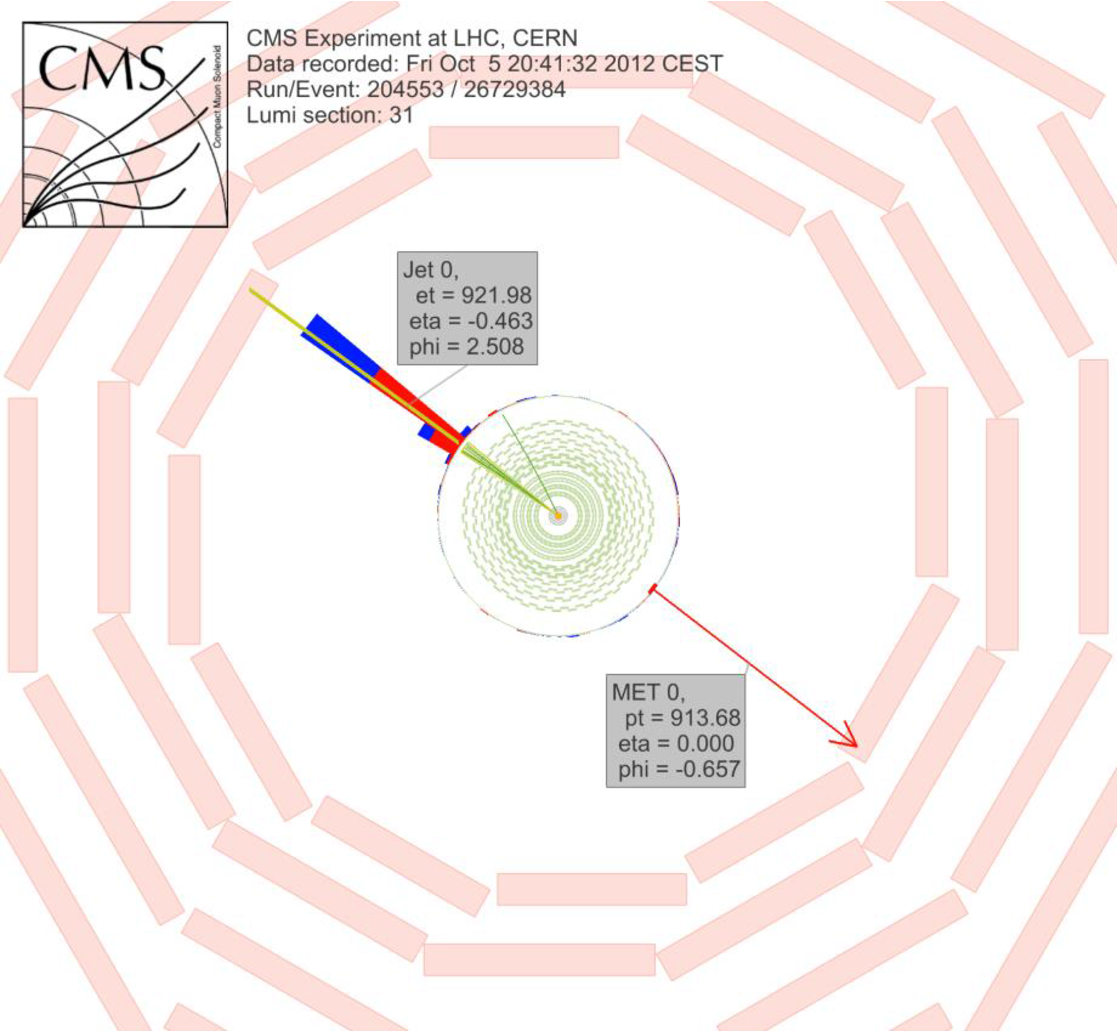
\includegraphics[width=.6\textwidth]{monojet_event.pdf} 
 \caption{Event display showing the monojet final state consisting of one jet and missing transverse momentum.}
 \label{fig:monojet_display}
\end{figure}

This trigger is studied using events passing the single electron trigger with a threshold of $p_T > \SI{23}{GeV}$, and applying an extra offline selection requiring an electron with $p_T > \SI{40}{GeV}$ passing the tight identification and a jet with $p_T > \SI{100}{GeV}$ and $|\eta| < 2.5$. The trigger efficiency is computed by determining the fraction of events which additionally pass the signal triggers, as a function of the hadronic recoil. The efficiency is above 98\% for events passing the analysis selection described in Section~\ref{sec:selection}, as shown in Figure~\ref{fig:trigger_eff}.

\begin{figure}[ht]
  \centering
 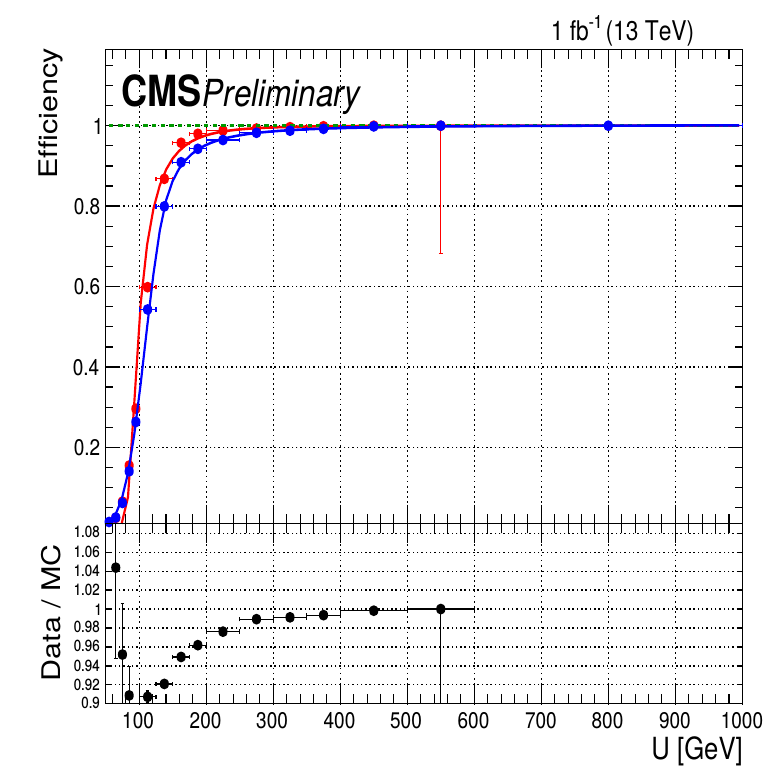
\includegraphics[width=.61\textwidth]{monojet_trigger.png} 
 \caption{The efficiency of the used signal triggers as a function of the hadronic recoil, in MC (red) and data (blue).}
 \label{fig:trigger_eff}
\end{figure}

To select events in the electron control regions, a single electron trigger was used with a threshold at $p_T > \SI{27}{GeV}$. The efficiency of this trigger is determined as a function of $p_T$ and $\eta$. This is done by ``tagging'' one electron with $p_T > \SI{40}{GeV}$ and $|\eta| < 2.1$ which passes the tight selection requirements. A second electron with $p_T > \SI{10}{GeV}$ and $|\eta| < 2.5$ is then selected, while the invariant mass of this pair is required to be between 60 and \SI{120}{GeV}, to correspond to the $Z$ boson mass. This tag-and-probe method ensures that backgrounds are removed and allows to measure the efficiency by simply taking the fraction of probes that passes the single electron trigger. The obtained trigger efficiency turn-on curves as a function of the electron transverse momentum are shown in Figure~\ref{fig:trigger_eff_e} for two $\eta$ bins, covering the \ac{ECAL} barrel and endcaps separately and leaving out the poorly instrumented region in between.

\begin{figure}[ht]
  \centering
 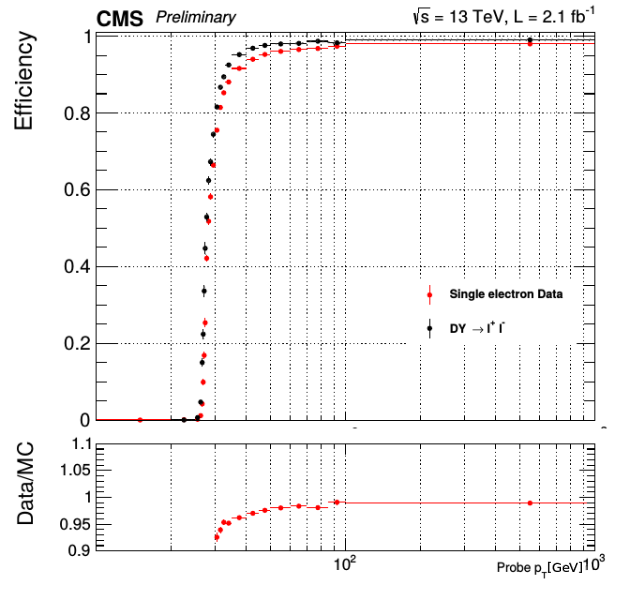
\includegraphics[width=.49\textwidth]{monojet_etrigger_1.png} 
 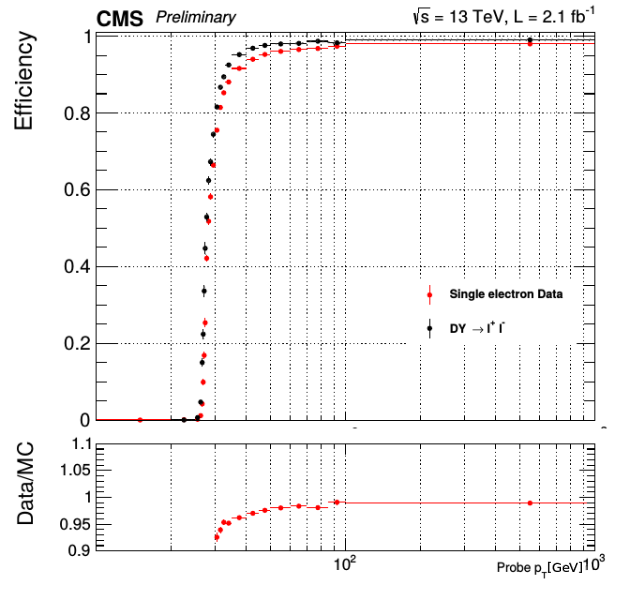
\includegraphics[width=.49\textwidth]{monojet_etrigger_1.png} 
 \caption{The efficiency of the single electron trigger in data (red) and MC (black) for $|\eta| < 1.4442$ (left) and $1.566 < |\eta| < 2.5$ (right).}
 \label{fig:trigger_eff_e}
\end{figure}

Finally, the events in the photon control region are selected with a single photon trigger requiring an isolated photon with $p_T > \SI{175}{GeV}$. The performance of this trigger is measured in data selected using a single photon trigger with a lower $p_T$ threshold, and the turn-on is shown in Figure~\ref{fig:trigger_eff_gamma}.

\begin{figure}[ht]
  \centering
 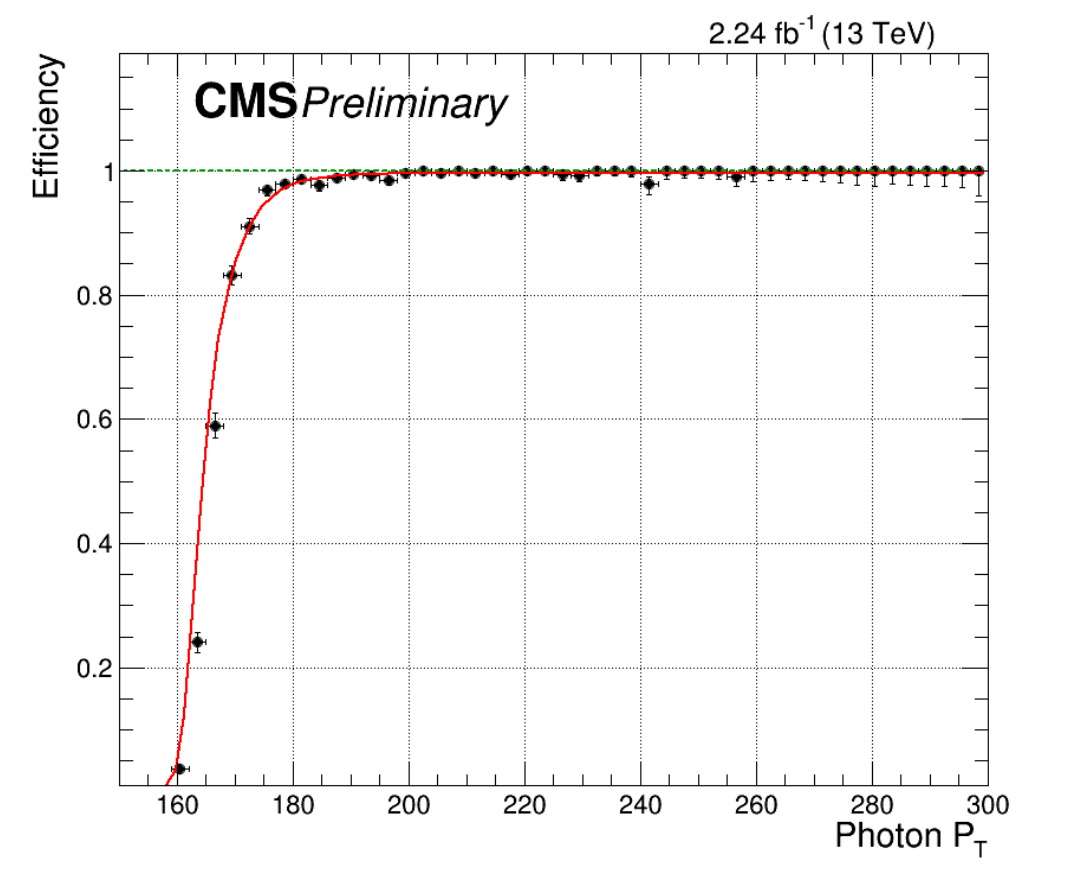
\includegraphics[width=.6\textwidth]{monojet_gammatrigger.png} 
 \caption{The efficiency of the single photon trigger measured in data.}
 \label{fig:trigger_eff_gamma}
\end{figure}

\section{Event selection}
\label{sec:selection}

Once the events have been fully reconstructed and the jets in the event have been corrected as described in Section~\ref{sec:jet_reconstruction}, an event selection is applied in order to efficiently select signal events and reduce the contribution from backgrounds, such as the production of a leptonically decaying $W$ boson in association with jets, semileptonic diboson decays, QCD multijets, and top quark production. The background contribution coming from events with a $Z$ boson produced together with a number of jets, where the $Z$ boson decays to two neutrinos, is irreducible as it produces exactly the same signature as the expected signal. The missing transverse momentum $E_T^{miss}$ is required to be larger than \SI{200}{GeV} in order to be safely above the trigger turn-on. Additionally, the leading jet is required to have $p_T > \SI{100}{GeV}$ in order to balance the missing transverse momentum, and $|\eta| < 2.5$. A cut on the difference in azimuthal angle between the $E_T^{miss}$ and the first four leading jets of $\Delta\phi(jet, E_T^{miss}) > 0.5$ is also applied. This is done to suppress the QCD background from mismeasurements of jet momentum or detector noise, which could introduce missing transverse momentum in the event, in the same direction as the mismeasured jet. The events are further cleaned by applying quality filters to remove events coming from beam or instrumental backgrounds. Finally, events containing a lepton, a photon, or a b-jet are vetoed as well. Figure~\ref{fig:MET} shows the $E_T^{miss}$ distribution for data and MC, after applying the described selection.

\begin{figure}[ht]
  \centering
 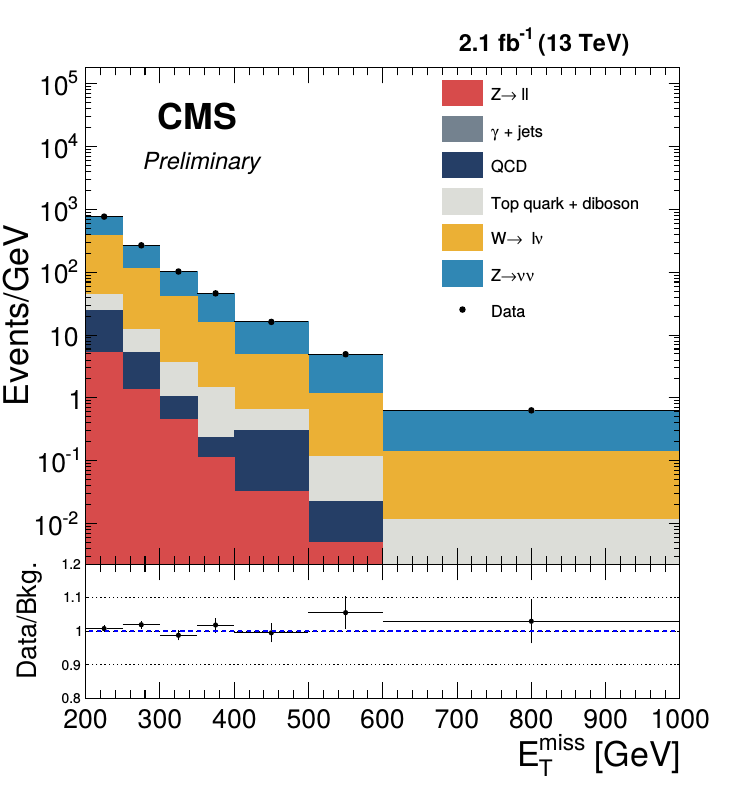
\includegraphics[width=.6\textwidth]{MET.png} 
 \caption{The missing transverse momentum distribution after applying the described event selection, for data and MC.}
 \label{fig:MET}
\end{figure}

Events containing a lepton are vetoed to suppress the electroweak backgrounds, such as $W(lv)$ + jets and semileptonic diboson decays, while the photon veto is added to suppress the $Z(\nu\nu)$ + photon + jets and $W(l\nu)$ + photon + jets background processes, and to ensure there is no overlap with a similar dark matter search which investigates the final state consisting of missing momentum and a photon. This rejects less than 1\% of the signal. Finally, the b-jet veto reduces the background from events with a single top quark or top quark pairs by a factor 3 and only reduces the signal by 5 to 10\%, depending on the type and mass of the mediator. No additional veto on the number of jets is applied.

\section{Background estimation}
\label{sec:bkgd}

% photon purity (2 methods):
% 
% lepton and photon eff: 2 methods

The dominant background comes from events with a $Z$ boson produced together with a number of jets, where the $Z$ boson decays to two neutrinos. This produces the same signature of jets with missing momentum as the signal, and results in an irreducible background. The second largest background consists of $W$ + jets events with a leptonically decaying $W$ boson. This background is already suppressed by the lepton veto, but a fraction of these events remain when the lepton is either not identified or outside of the detector acceptance. The remaining background events come from top quark decays, which are suppressed by the b-jet veto, semileptonic diboson ($WW$, $WZ$, and $ZZ$) decays, and QCD multijet events. The two main background contributions are estimated from five control regions in data consisting of dimuon, dielectron, single muon, single electron, and photon + jets events.  The contributions from top quark decays and semileptonic diboson decays are estimated using simulated samples, while the QCD multijet background is estimated using a data-driven approach.

\subsection{The \textit{Z} and \textit{W} background estimation}
\label{sec:main_bkgd}

The traditional control region for the $Z$ boson background is the dimuon control region. This region is dominated by $Z\rightarrow\mu\mu$ events, which are very similar to the $Z(\nu\nu)$ + jets background events, the only difference being the decay mode. The production mode and kinematics in the control region are very similar, as well as the acceptance. However, the branching ratio of the $Z$ boson decaying into two muons is 6 times smaller than the branching ratio for the decay to two neutrinos. As a result of this, and due to the muon selection efficiency, the dimuon control region contains about 10 times less $Z$ boson events than the signal region. In order to improve this statistical limitation, other control regions have been added as well.

The yield of $Z(\nu\nu)$ and $W(l\nu)$ + jets events in the signal region is therefore estimated from five control regions by using the ratio between data and MC in the control region, per bin of the hadronic recoil distribution. As illustrated in Figure~\ref{fig:CR}, the $W(l\nu)$ + jets background is estimated from the single lepton control regions, and the $Z(\nu\nu)$ + jets background is predicted from the dilepton and photon + jets control regions. Five transfer factors are therefore needed to connect the control regions to the signal region. An additional transfer factor is used between the $Z(\nu\nu)$ + jets and $W(l\nu)$ + jets backgrounds to factor in the experimental as well as theoretical correlations between these two backgrounds. 

\begin{figure}[ht]
  \centering
 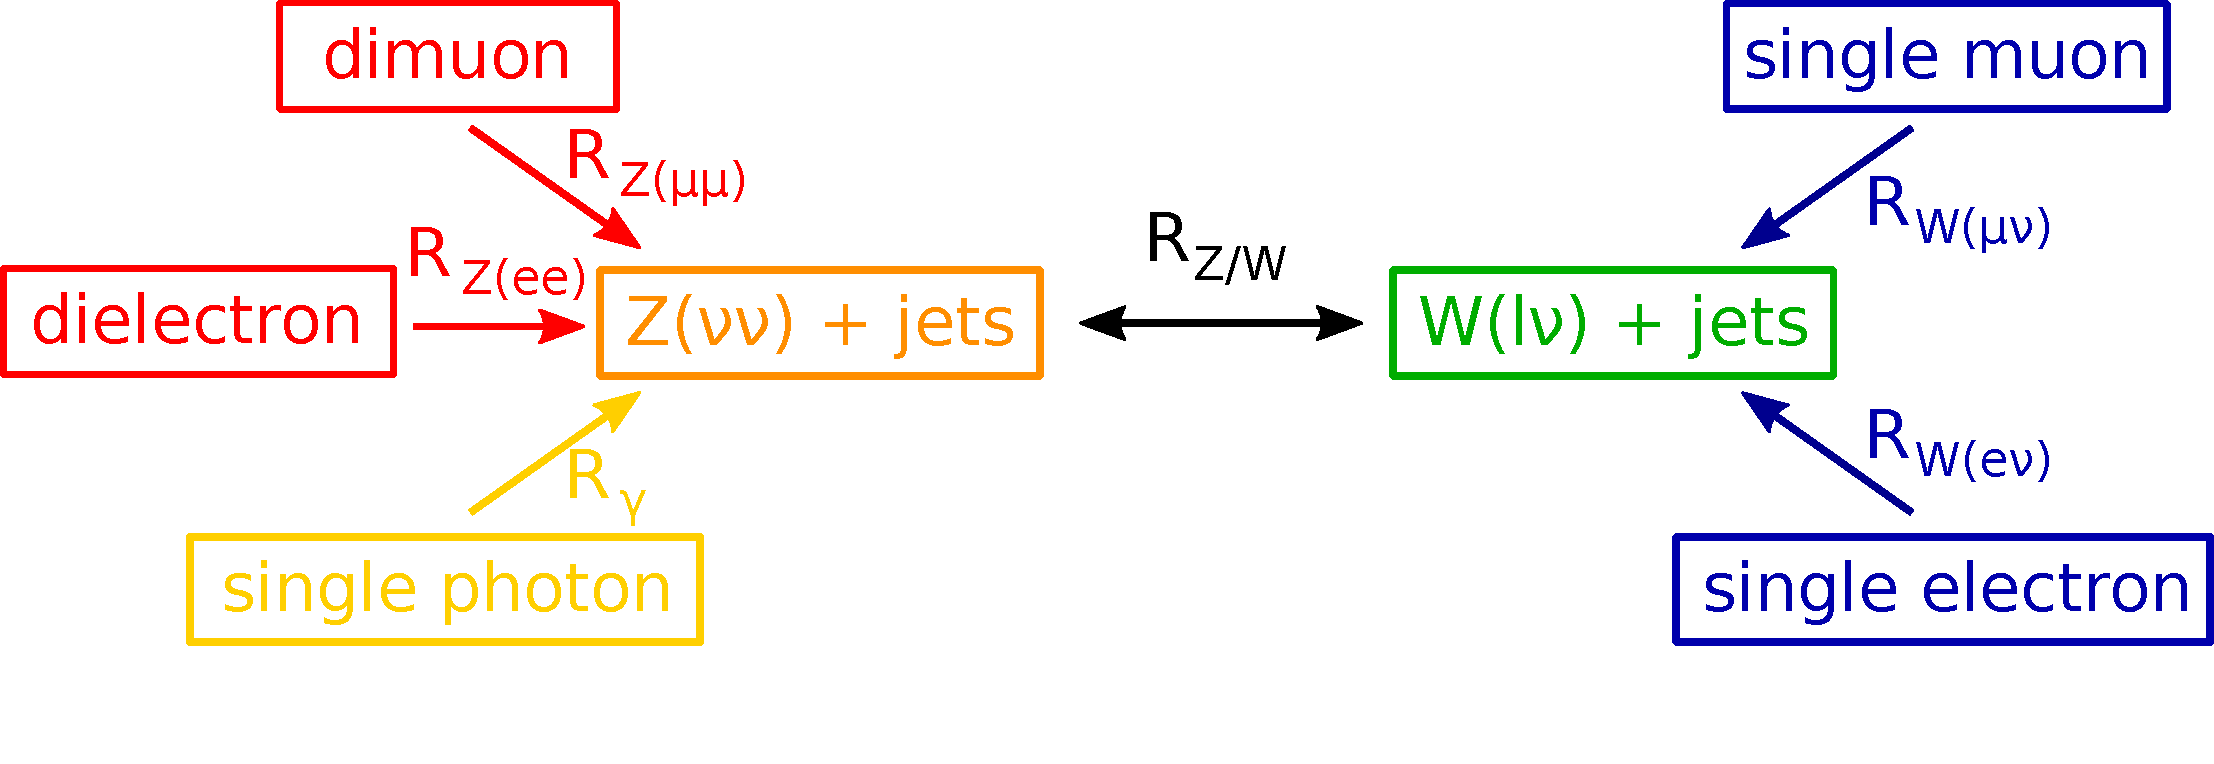
\includegraphics[width=\textwidth]{bkgd_estimation.pdf} 
 \caption{Schematic overview of the five control regions used to estimate the $Z(\nu\nu)$ and $W(l\nu)$ + jets backgrounds with the transfer factors.}
 \label{fig:CR}
\end{figure}

For the prediction using $Z\rightarrow \mu\mu$ events in the dimuon control region for example, the predicted yield of $Z\rightarrow\nu\nu$ events is given by
\begin{align}
 N_{Z(\nu\nu)} &= \frac{N_{Z(\mu\mu)}^{data}}{N_{Z(\mu\mu)}^{MC}}\ N_{Z(\nu\nu)}^{MC}\\
 &= \frac{N_{\mu\mu}^{data} - N_{Bkgd}}{N_{Z(\mu\mu)}^{MC}}\ N_{Z(\nu\nu)}^{MC} \\
 &= \left(N_{\mu\mu}^{data} - N_{Bkgd}\right)\ R_{Z(\mu\mu)},
\end{align}
where the number of $Z(\mu\mu)$ + jets events in data $N_{Z(\mu\mu)}^{data}$ is given by the number events in the dimuon sample, removing the number of background events, and $N_{Z(\mu\mu/\nu\nu)}^{MC}$ represent the number of $Z(\mu\mu/\nu\nu)$ + jets events in MC. The five transfer factors, denoted by $R$, are derived from simulation and take into account the impact of lepton acceptance and efficiency, as well as the additional $E_T^{miss}$ requirement for the single electron control region. They also include the difference in branching ratio and the relation between the differential cross sections of the photon, $W$, and $Z$ boson production as a function of the boson $p_T$. The transfer factors are computed as a function of the hadronic recoil, and are shown in Figure~\ref{fig:TF}. Furthermore, the $Z/W$ ratio shown in the bottom right plot of Figure~\ref{fig:TF} provides an additional constraint between the $Z(\nu\nu)$ + jets and $W(l\nu)$ + jets backgrounds.

\begin{figure}[p]
  \centering
 \vspace{.3cm}
 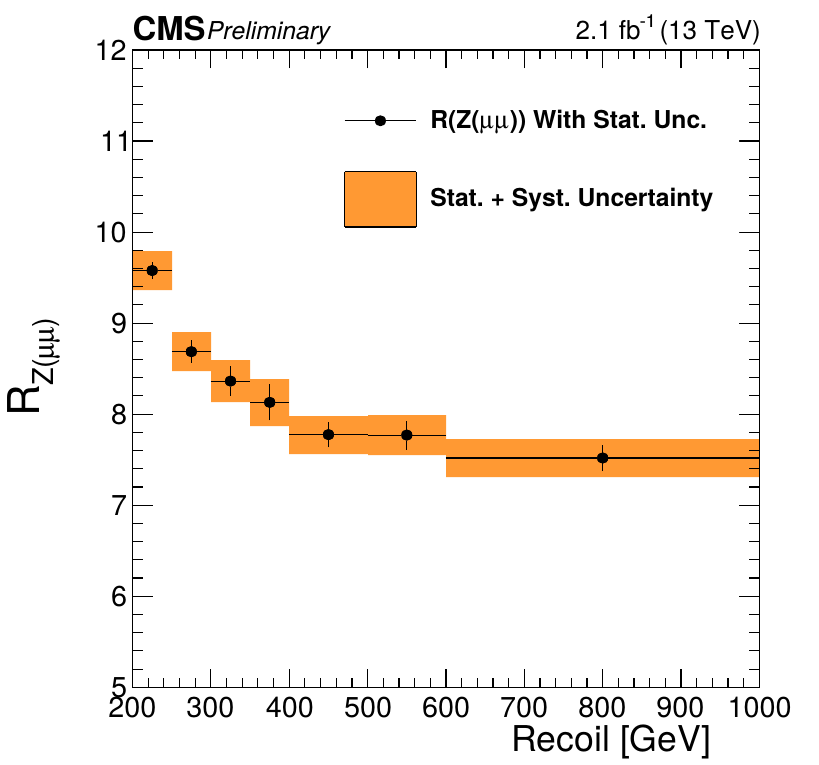
\includegraphics[width=.48\textwidth]{dimuon_TF.png} 
 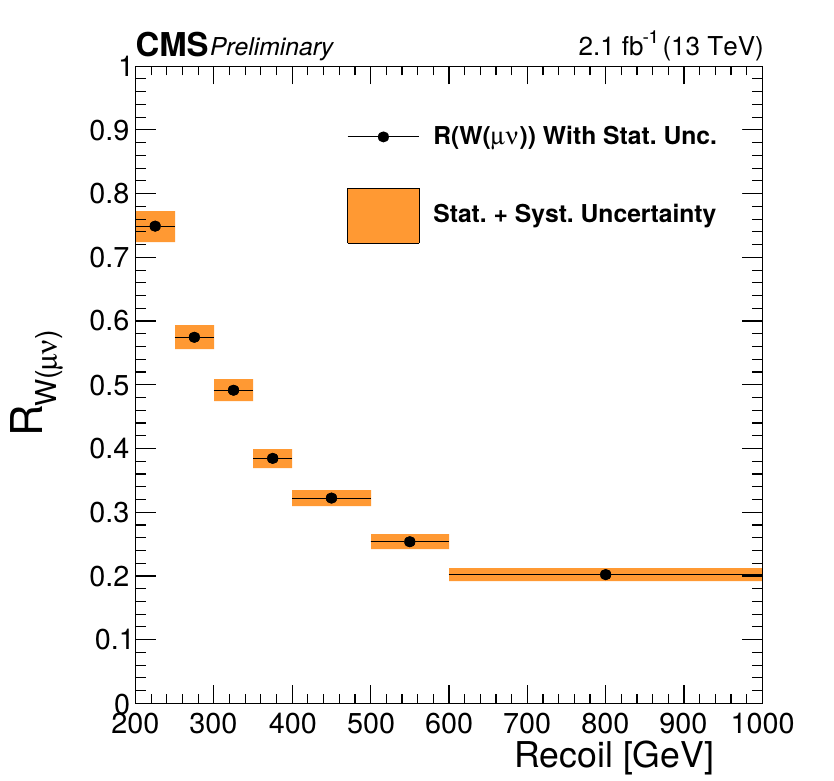
\includegraphics[width=.49\textwidth]{single_muon_TF.png} \\
 \vspace{.4cm}
 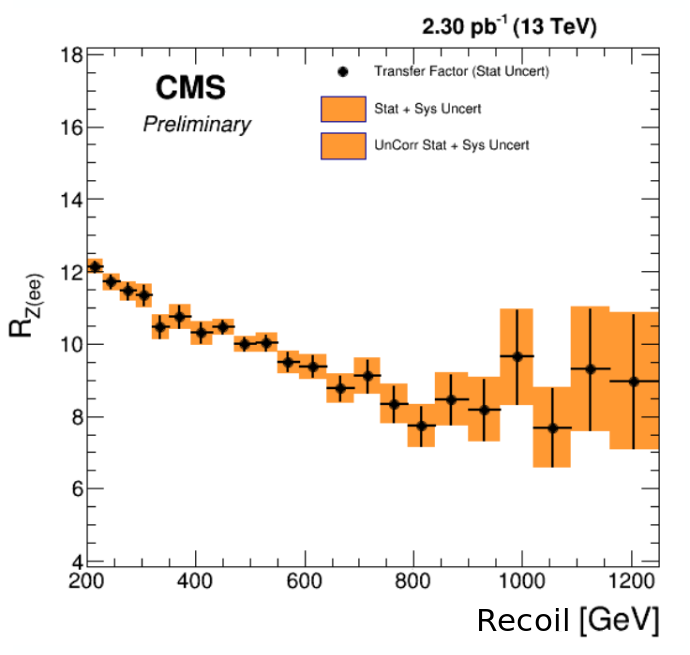
\includegraphics[width=.48\textwidth]{dielectron_TF.png} 
 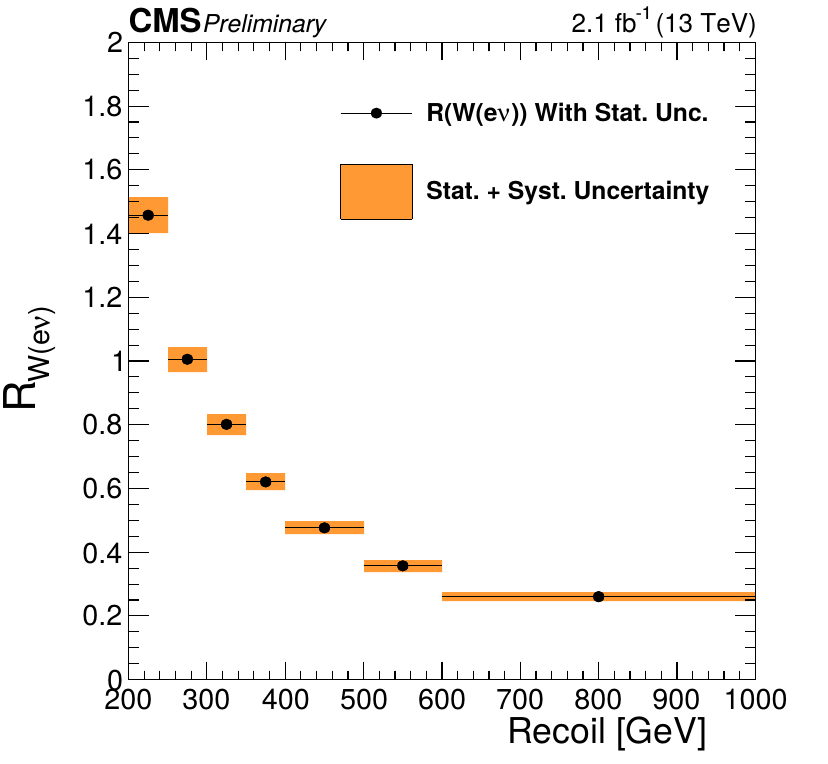
\includegraphics[width=.49\textwidth]{single_electron_TF.png} \\
 \vspace{.2cm}
 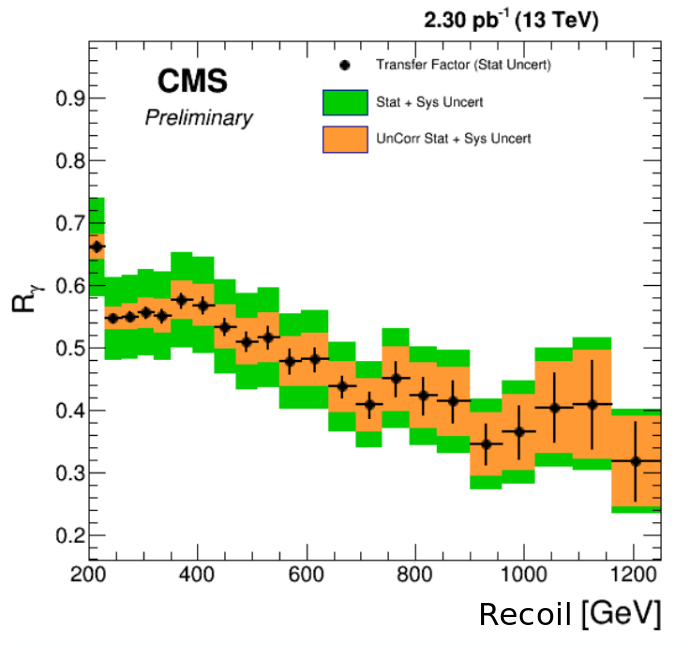
\includegraphics[width=.48\textwidth]{gamma_TF.png} 
 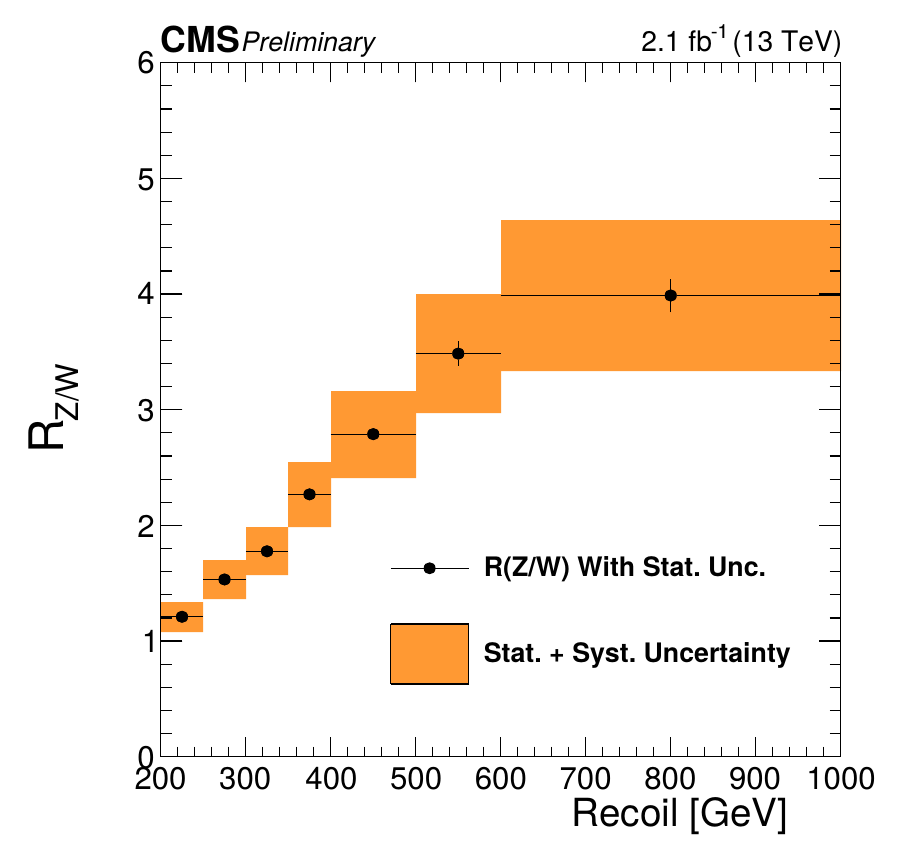
\includegraphics[width=.49\textwidth]{ZW_ratio.png} 
 \caption{Transfer factors for the dimuon (top left), single muon (top right), dielectron (middle left), single electron (middle right), and photon + jets (bottom left) control regions. The ratio of the $Z$ and $W$ transfer factors is shown in the bottom right plot.}
 \label{fig:TF}
\end{figure}

The simulated samples used for the background estimation are generated at leading order (LO) using the \textsc{Madgraph} generator, and corrected to next-to-leading order (NLO). These corrections are crucial in order correctly represent the data since inclusively, the simulation is approximately 40\% higher than the data when using only LO calculations. The NLO QCD k-factors are derived from samples generated at NLO with \textsc{MadGraph5\_}a\textsc{MC@NLO}, while the \ac{NLO} electroweak k-factors are obtained from theoretical calculations~\cite{Kuhn:2005gv, Kallweit:2015fta, Kallweit:2014xda, Kallweit:2015dum}. The differential cross section as a function of the boson $p_T$ is shown in Figure~\ref{fig:kfactors} for photon, $W$, and $Z$ production, and the obtained k-factors are displayed in the ratio plots. More details on the different control regions are given in the following.

\begin{figure}[p]
  \centering
 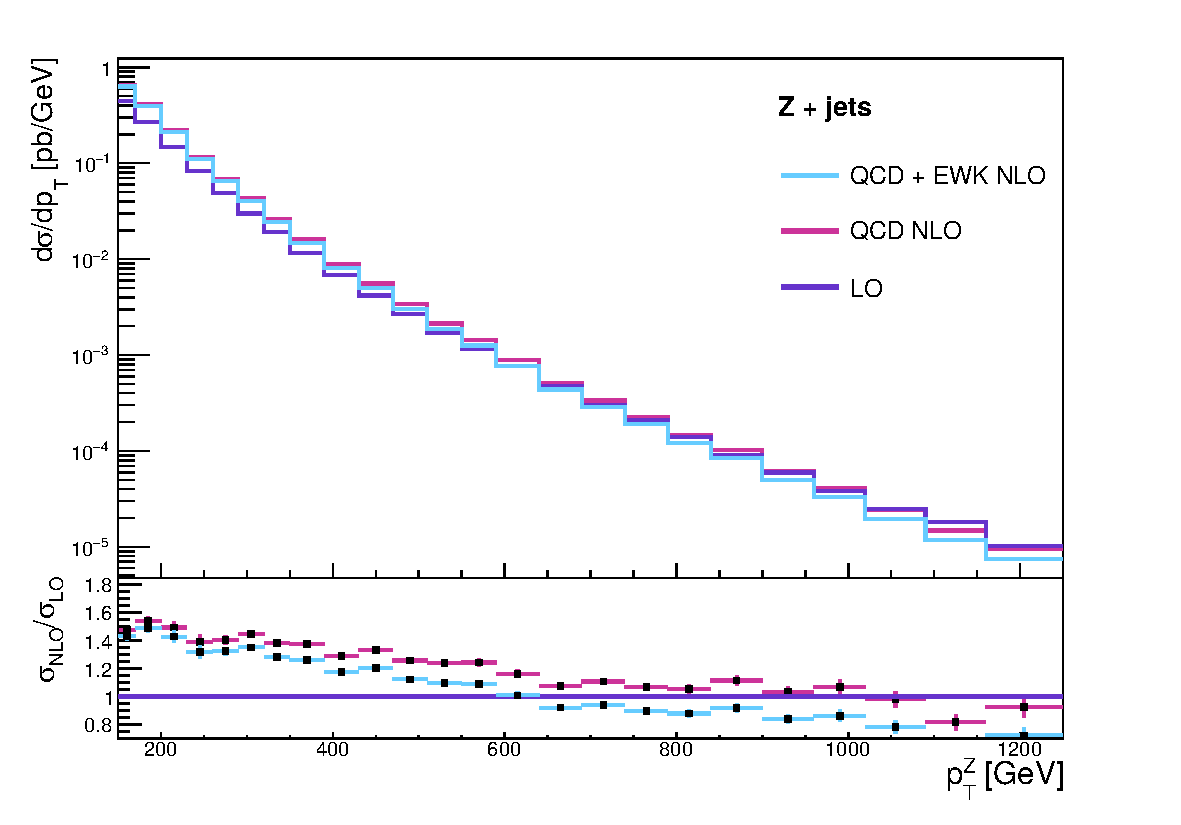
\includegraphics[width=.7\textwidth]{Z_EWK_kfactor.pdf} 
 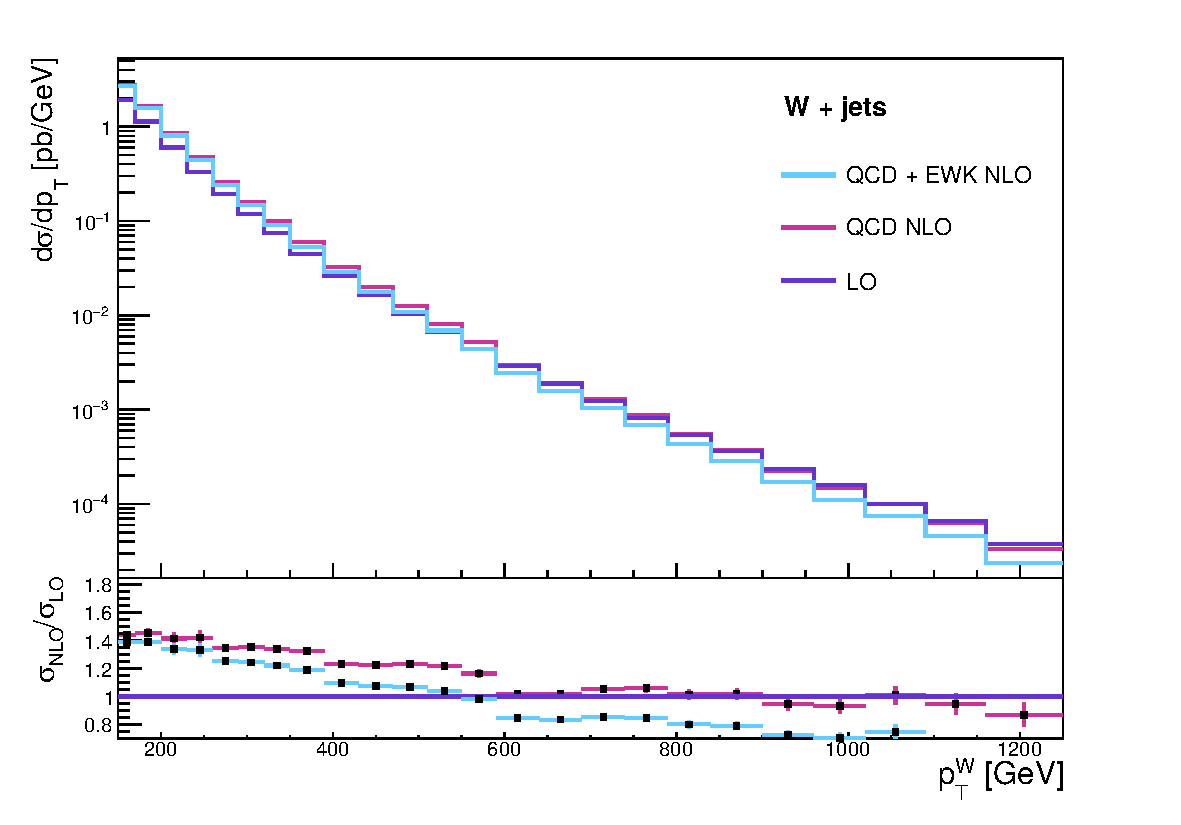
\includegraphics[width=.7\textwidth]{W_EWK_kfactor.pdf} \\
 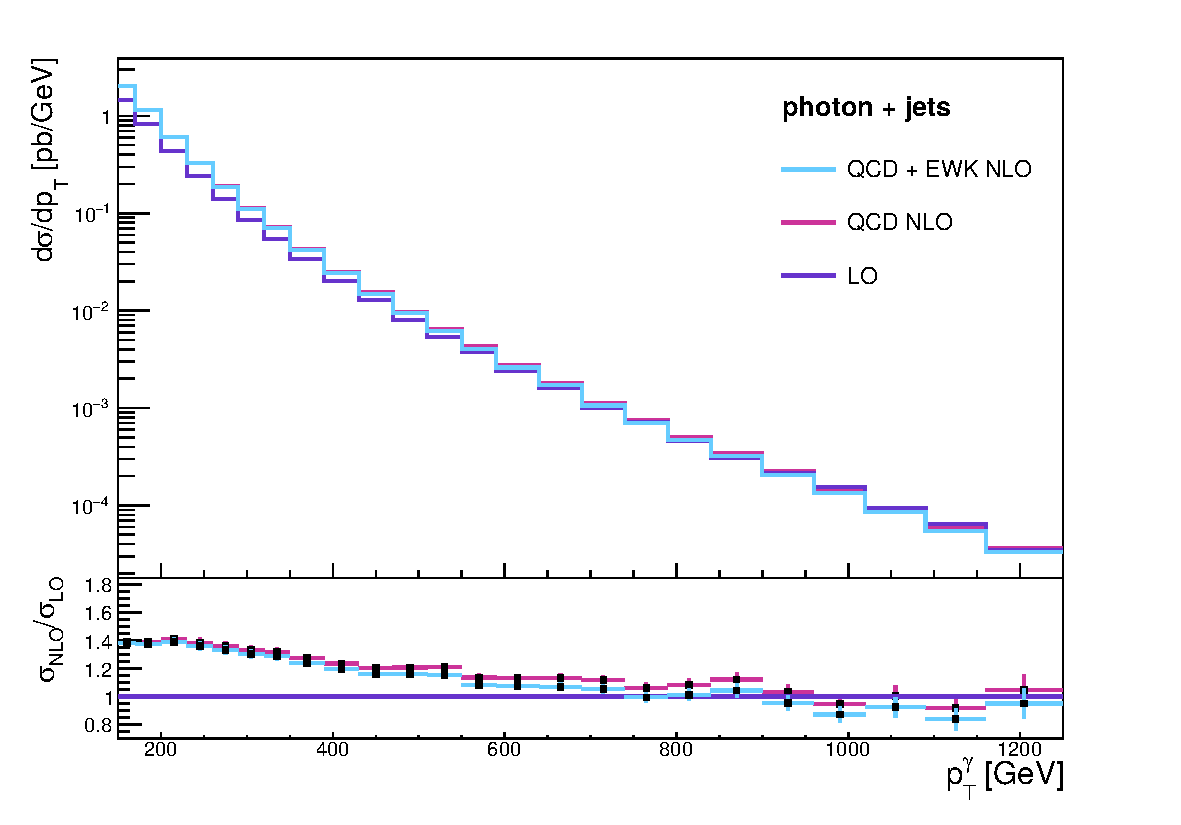
\includegraphics[width=.7\textwidth]{gamma_EWK_kfactor.pdf} 
 \caption{The differential cross section as a function of the boson $p_T$ for photon, $W$,and $Z$ production, using boson $p_T$-binned \ac{NLO} samples. The resulting k-factors are shown in the ratio plots.}
 \label{fig:kfactors}
\end{figure}

\begin{itemize}
 \item[] \textbf{Dimuon control region}\\ In the dimuon control region the events are selected using the monojet triggers and applying the same requirements as described in Section~\ref{sec:selection} for the signal region, using the hadronic recoil instead of the missing transverse momentum, except for the muon veto. Additionally, exactly two muons with opposite charge should be identified using the loose identification, and at least one should also pass the tight selection requirements. The leading muon should have a transverse momentum larger than \SI{20}{GeV}, and the second one should have $p_T > \SI{10}{GeV}$. Finally, the dimuon mass should be between 60 and \SI{120}{GeV}, corresponding to the $Z$ boson mass.

\item[] \textbf{Single muon control region}\\ In order to model the second largest background, coming from $W(l\nu)$ + jets events, a single muon control region is used. This control region is in addition also used to constrain the $Z(\nu\nu)$ + jets background. The events in the single muon control region are required to pass the monojet triggers and event selection replacing the $E_T^{miss}$ by the hadronic recoil obtained by removing the muon, except for the muon veto. One muon should then pass the tight selection requirements and have $p_T > 20$~GeV.

\item[] \textbf{Dielectron control region}\\ The dielectron control region is also used to constrain the $Z\rightarrow\nu\nu$ background. The events are selected by the single electron triggers. Similarly to the dimuon control region, the events are required to pass the monojet selection, except for the electron veto. Instead, exactly two electrons with $p_T > 10$~GeV are required to pass the loose identification described in Section~\ref{sec:electron_ID}. In addition, at least one electron should pass the tight selection requirements, and the leading electron is required to have $p_T > 40$~GeV in order to have a high probability to have passed the single electron trigger. Finally, the dielectron mass should be between 60 and 120~GeV, in order to be consistent with a $Z$ boson decay. The jump that can be observed in the last bin of the resulting transfer factor in the middle left plot of Figure~\ref{fig:TF} is due to the isolation requirement of the single electron trigger. This was verified by removing the trigger selection in MC, yielding a flat transfer factor.

\item[] \textbf{Single electron control region}\\ The single electron control region is used to constrain the $W(l\nu)$ + jets background. In the single electron control region, the events are required to have one electron with $p_T > 40$~GeV passing the tight selection requirements, analogous to the single muon control region. In this region, a large amount of QCD background is however present due to jets being wrongly reconstructed as electrons. In order to reject most of those events, an additional cut on the $E_T^{miss}$, which includes the single electron, is added at 50~GeV. This reduces the QCD background by an order of magnitude.

\item[] \textbf{Photon + jets control region}\\Due to its large yield, the photon + jets control region provides the dominant constraint on the high-$p_T$ part of the $Z(\nu\nu)$ + jets background. The selection of these events is done using the single photon triggers and applying the monojet selection, except for the photon veto. One photon is then required to pass the tight identification and to have $p_T > 175$~GeV. Additionally, it should be reconstructed inside the \ac{ECAL} barrel ($|\eta| < 1.4442$) in order to achieve a high purity of at least 95\%. Events with more than one photon passing the loose identification requirements described in Section~\ref{sec:electron_ID} are rejected.
\end{itemize}

\subsection{The QCD background estimation}

While QCD multijet background events are generally well balanced in the transverse plane, missing transverse momentum can arise in the event due to jet energy mismeasurements, punch-through\footnote{It can happen that a jet is not fully contained inside the calorimeters, and leaks into the muon system. In that case, part of the energy of the jet is lost, leading to missing transverse momentum.}, uninstrumented or defective regions in the detector, hot spots, or neutrinos from decays of heavy-flavour mesons. Although these effects will very rarely yield a large missing transverse momentum, the QCD production cross section is very large compared to other processes, and some events can be selected at high missing transverse momentum. The event selection detailed in Section~\ref{sec:selection} was designed to suppress contributions from the QCD multijet background, reducing it to the percent level. However, this background is not well reproduced in the simulation, and thus requires a background estimation using a data control region.

The yield is predicted using 
%by combining two different approaches, namely the ``rebalance and smear'' technique and the $\Delta\phi$ extrapolation method. The rebalance and smear technique minimises the missing transverse momentum through a kinematic using the jet resolutions. The event is then rebalanced by varying each jet and the remaining hadronic recoil within their computed uncertainties. The resulting jets are then smeared with the measured jet resolution, and the prediction for the QCD $E_T^{miss}$ distribution is obtained. The used data for this method are selected based on jets and applying a cut on the $H_T$ present in the event. 
the $\Delta\phi$ extrapolation method. This is done by estimating the QCD background in data selected using the signal triggers and applying the event selection, but inverting the $\Delta\phi$ selection cut and instead requiring $\min\Delta\phi(jet, E_T^{miss}) < 0.5$. An extrapolation is then made to the signal region using transfer factors derived from simulated events generated at \ac{LO} with \textsc{MadGraph} in several bins of $H_T$. The obtained estimation using this method yields a contribution that is a factor 2 larger than the prediction from simulation, 
%which agrees well with the the rebalance and smear technique, 
as can be seen in Figure~\ref{fig:QCD_prediction}.

\begin{figure}[ht]
  \centering
 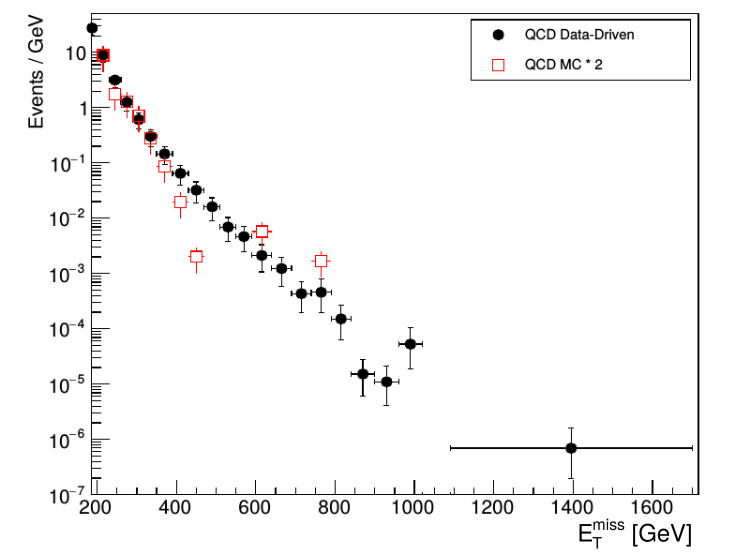
\includegraphics[width=.7\textwidth]{QCD_prediction.png} 
%  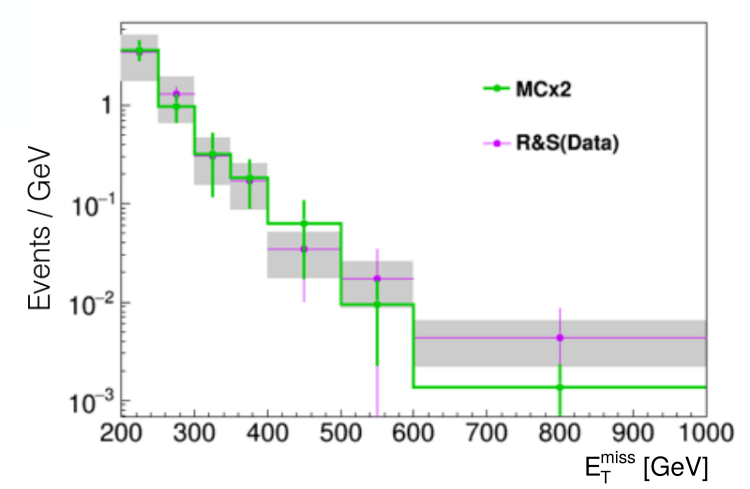
\includegraphics[width=.52\textwidth]{rebalanceandsmear.png} 
 \caption{Predicted $E_T^{miss}$ distribution of the QCD multijet background obtained using the $\Delta\phi$ extrapolation method, using data (black) and MC simulations (red). The simulation is scaled by a factor~2.}
 \label{fig:QCD_prediction}
\end{figure}

% how is it combined exactly?

\subsection{Simulation-based background estimation}

Contributions are also expected from diboson production, from top quark decays, both from $t\bar{t}$ and single top production, and from $Z(ll)$ + jets events where the leptons are not detected. These backgrounds are estimated from MC simulations. 

Top quarks typically decay into a $W$ boson and a $b$ quark. When the $W$ boson decays leptonically, a neutrino is produced, generating genuine missing transverse momentum. If the event is not removed by the b-jet veto and the lepton is not identified, this type of events contributes to the background in the signal region. However, due to the small production cross section and the applied event selection, only a small fraction of these events are selected. In order to estimate the contribution of this background, a $t\bar{t}$ sample has been produced at \ac{LO} with \textsc{MadGraph}, and single top events were generated with \textsc{PowHeg} at \ac{NLO}.

When one of the weak bosons produced in diboson events decays leptonically, generating one or more neutrinos, and the other one decays hadronically, jets and missing transverse momentum are produced. The samples used to estimate this background have been produced using \textsc{Pythia}.

Finally, when the leptons in $Z(ll)$ + jets events are lost or out of the detector acceptance, these events can mimic the monojet signature as well. MC samples have been generated at \ac{LO} using \textsc{MadGraph} in several bins of $H_T$ in order to estimate the contribution from this sub-dominant background.

\section{Systematic uncertainties}
\label{sec:syst}

For the main backgrounds, multiple systematic uncertainties on the transfer factors are taken into account. Systematic uncertainties are added for the selection efficiency of muons, electrons, tau leptons, and photons, and for the photon purity in the photon + jets sample. Additionally, systematic uncertainties are added to take into account the electron and photon triggers. These uncertainties are fully correlated across the bins in recoil. The uncertainty on the modelling of the $E_T^{miss}$ is dominated by the jet energy scale uncertainty, varying between 3 and 5\%.

Uncertainties are also added from theory, to take into account variations of the factorisation and renormalisation scales, PDF uncertainties, and the NLO electroweak corrections~\cite{Kuhn:2005gv, Kallweit:2015fta, Kallweit:2014xda, Kallweit:2015dum}. The former 3 uncertainties are shown in Figure~\ref{fig:kfactors_unc} for the $Z$ + jets, $W$ + jets, and photon + jets samples. The  uncertainties are then propagated to the transfer factors, and are displayed in Figure~\ref{fig:transfer_factors_unc}. To evaluate the PDF uncertainty, the samples are reweighted with event-by-event scale factors representing the shift in the kinematic distributions from variations in the PDF. The transfer factors are then produced for each variation, and the RMS of the variation is taken as PDF uncertainty. Similarly, the renormalisation and factorisation scales are varied up and down by a factor 2, and the uncertainties are derived from the resulting transfer factors. For the electroweak corrections, the full correction is taken as an uncertainty.

\begin{figure}[ht]
  \centering
 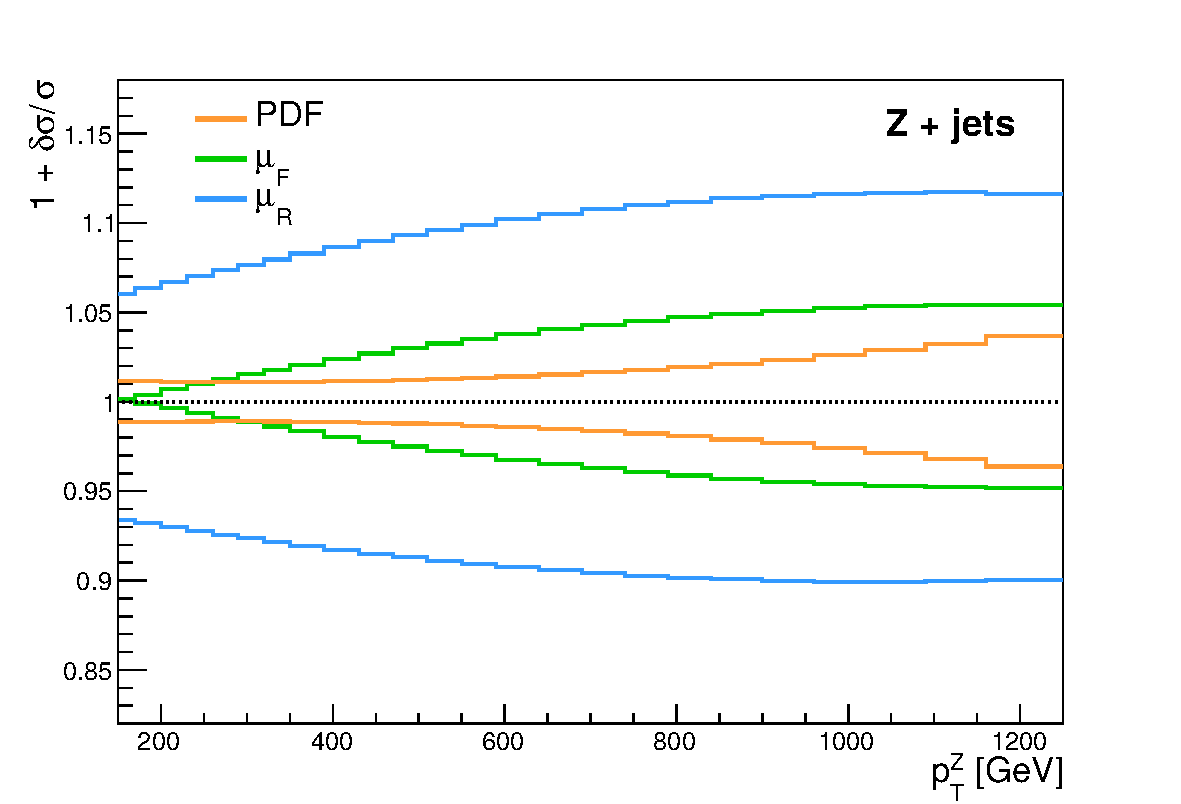
\includegraphics[width=.49\textwidth]{Z_uncertainties_smooth.pdf} 
 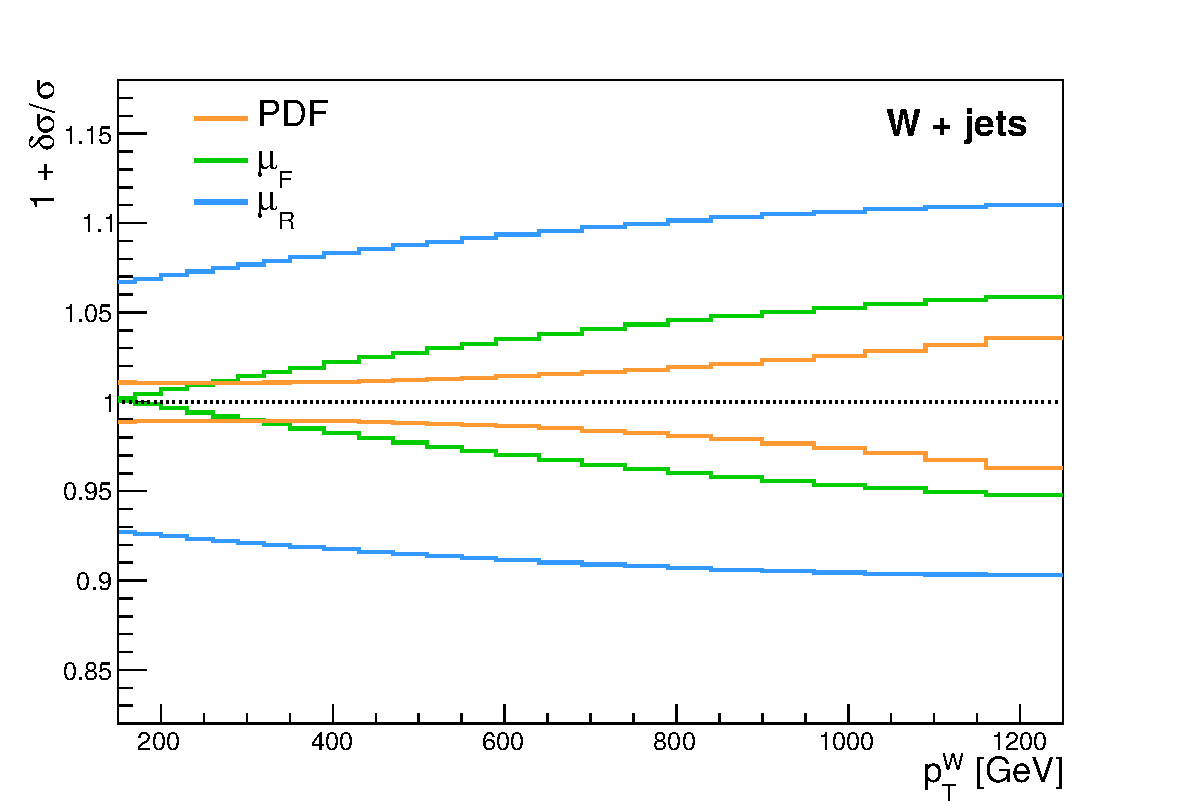
\includegraphics[width=.49\textwidth]{W_uncertainties_smooth_new.pdf} \\
 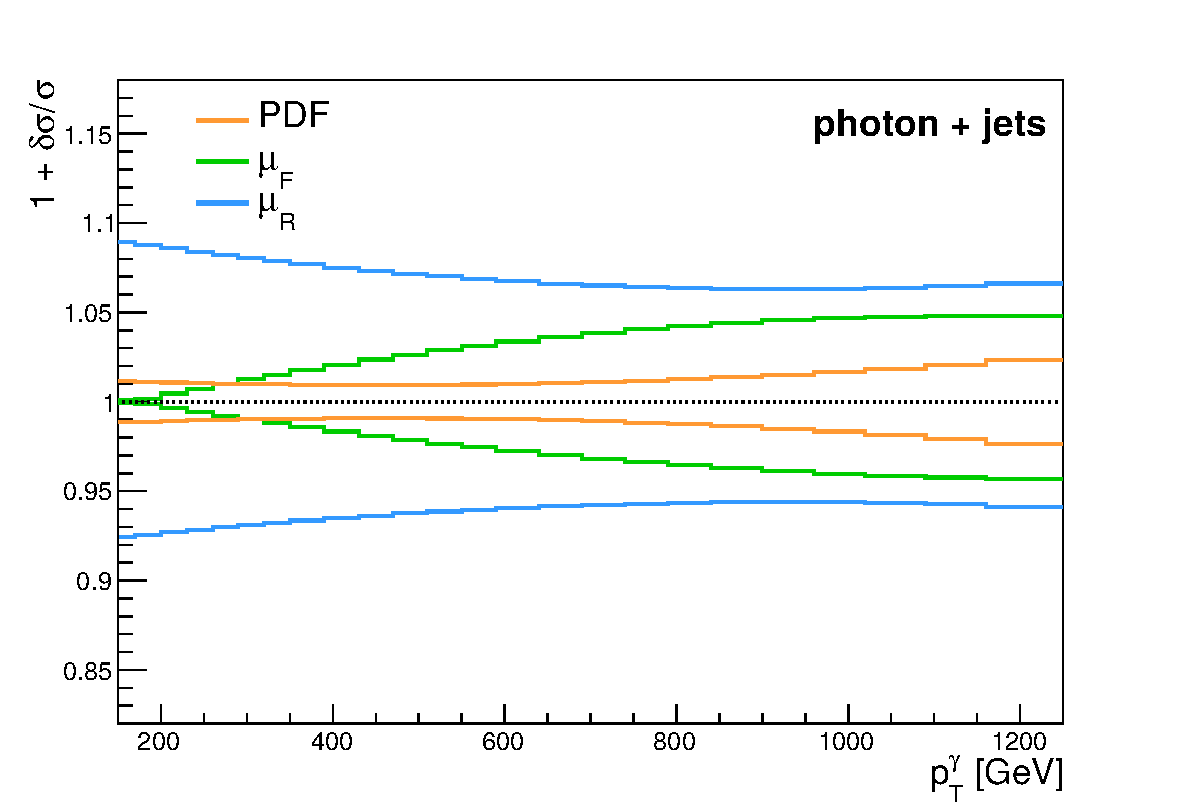
\includegraphics[width=.49\textwidth]{gamma_uncertainties_smooth.pdf} 
 \caption{The PDF, renormalisation, and factorisation scale uncertainties for the $Z$ + jets (top left), $W$~+~jets (top right), and photon + jets (bottom) samples. The uncertainties from the renormalisation and factorisation scales are obtained by separately varying them up and down by a factor 2.}
 \label{fig:kfactors_unc}
\end{figure}

\begin{figure}[ht]
  \centering
 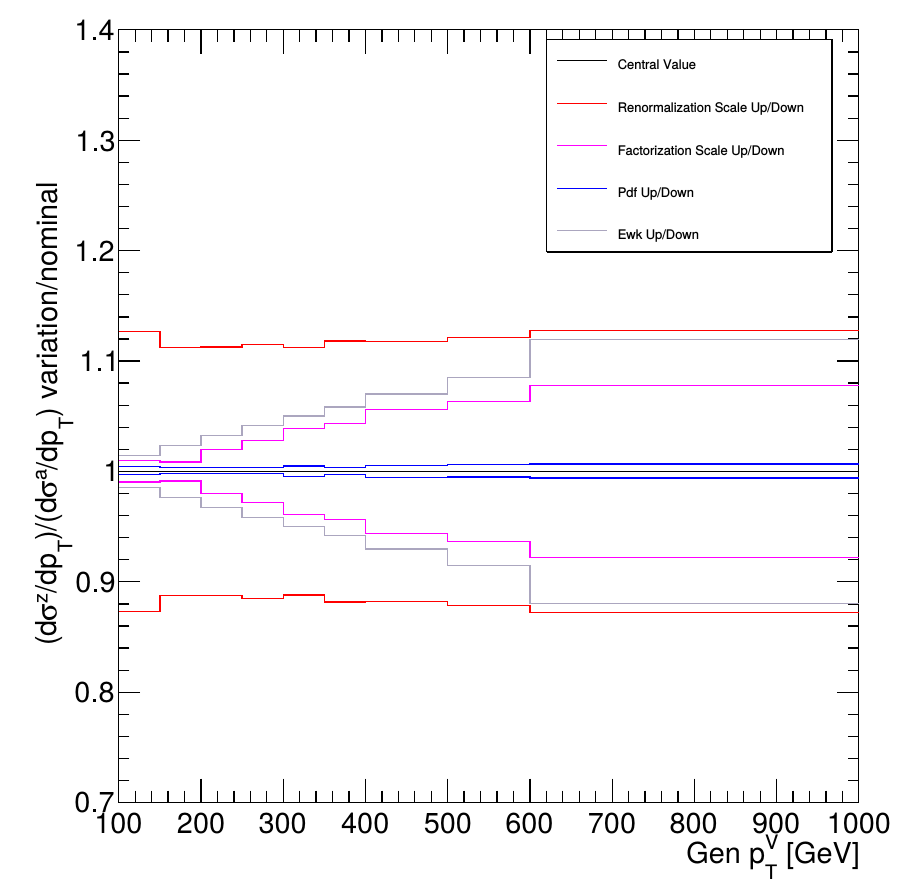
\includegraphics[width=.49\textwidth]{syst1.png} 
 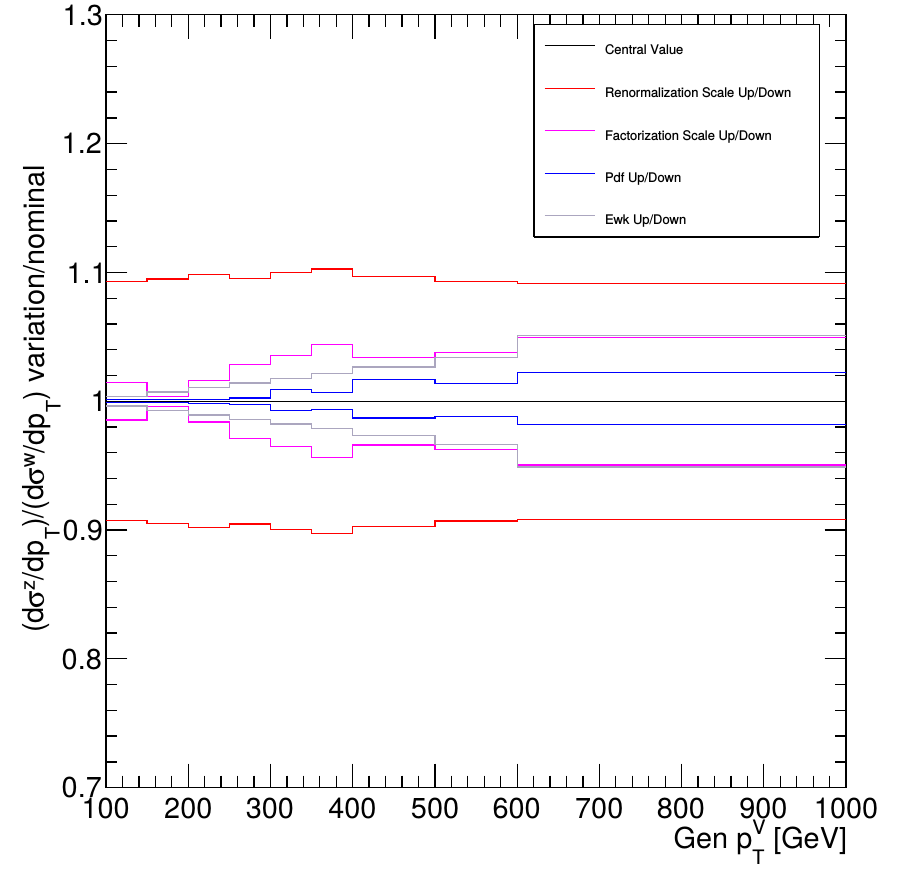
\includegraphics[width=.49\textwidth]{syst2.png}
 \caption{The theoretical uncertainties on the $Z/\gamma$ (left) and $Z/W$ (right) transfer factors, showing the renormalisation and factorisation scale uncertainties, the \ac{PDF} uncertainty, and the uncertainty from electroweak corrections.}
 \label{fig:transfer_factors_unc}
\end{figure}

The overall uncertainty on the QCD background varies between 50\% and 150\% depending on the $E_T^{miss}$ region, and includes variations in the jet response and the statistical uncertainty on the transfer factors. The remaining subdominant top quark and diboson backgrounds are obtained directly from simulation. A systematic uncertainties  of 20\% is taken into account for the uncertainty on the production cross section of these processes. Additionally, a systematic uncertainty is added due to the uncertainty on the b-tagging applied for the b-jet veto, which amounts to 6\% for the top quark background an 2\% for the diboson background. The uncertainty on the modelling of the $E_T^{miss}$ in simulation varies between 2\% and 5\%, depending on the $E_T^{miss}$. Finally, a systematic uncertainty of 2.7\%~\cite{CMS:2016eto} is added for all backgrounds derived from MC simulations, to take into account the uncertainty on the luminosity measurement.

Lastly, for the signal models described in Section~\ref{sec:monojet_models} and simulated as summarised in Section~\ref{sec:monojet_sim}, systematic uncertainties are included for the luminosity measurement (2.7\%), the b-jet veto (2\%), and the modelling of the $E_T^{miss}$ distribution in simulation (2\% to 5\%). The systematic uncertainties coming from variations of the factorisation and renormalisation scales and PDF uncertainties amount to 20\% for the vector and axial-vector signal samples and 30\% for the scalar and pseudoscalar signals.

\section{Results}
\label{sec:results}

The results are extracted by performing a binned fit to the missing momentum spectrum, fitting simultaneously over the five control regions and the signal region, under a given signal hypothesis. This is done using the $CL_S$ criterion~\cite{CLS1,CLS2} in the asymptotic approximation, described in Section~\ref{sec:limits}, using the RooStat-based~\cite{Moneta:2010pm} Combine tool~\cite{combine}. The systematic uncertainties described in Section~\ref{sec:syst} are modelled as nuisance parameters and their uncertainties are propagated as shape and normalization variations of the $Z(\nu\nu)$ + jets and $W(l\nu)$ + jets background. In Figure~\ref{fig:nuisance}, the nuisance parameters and their normalised uncertainties are shown before and after the fit to the data in the control regions. Before the fit they are all centred at 0 and have an uncertainty of 1. After the fit, the two largest deviations originate from the statistical uncertainty on the $Z/W$ transfer factor and the uncertainty on the muon scale factor, but no significant tension is present in the fit and most nuisance parameters are not biased or constrained by the fit.
The photon + jets control region, which has the largest yields, drives the fit and the post-fit prediction therefore corresponds well to the data. A good agreement is obtained in all control regions, and the overall change in the transfer factors is less than 10\%.

\begin{figure}[ht]
  \centering
 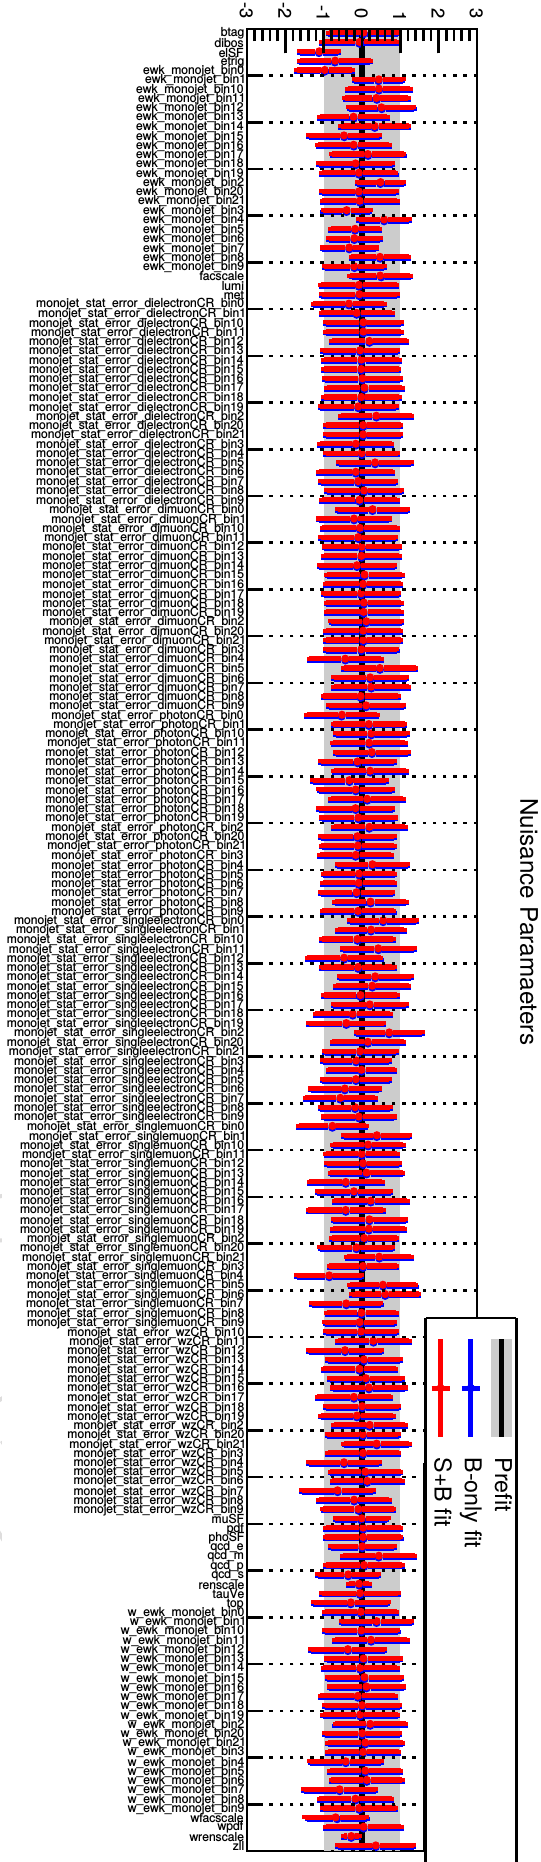
\includegraphics[width=.44\textwidth]{nuisance_new.png} 
 \caption{The post-fit nuisance parameters and their uncertainties, compared to the pre-fit values.}
 \label{fig:nuisance}
\end{figure}

% Figures~\ref{fig:postfit_1} and \ref{fig:postfit_2} show the hadronic recoil distributions in the different control regions, before and after the fit. The photon + jets control region, which has the largest yields, drives the fit and the post-fit prediction therefore corresponds well to the data. A good agreement is observed in all control regions, and the overall change in the transfer factors is less than 10\%.

% \begin{figure}[p]
%   \centering
%  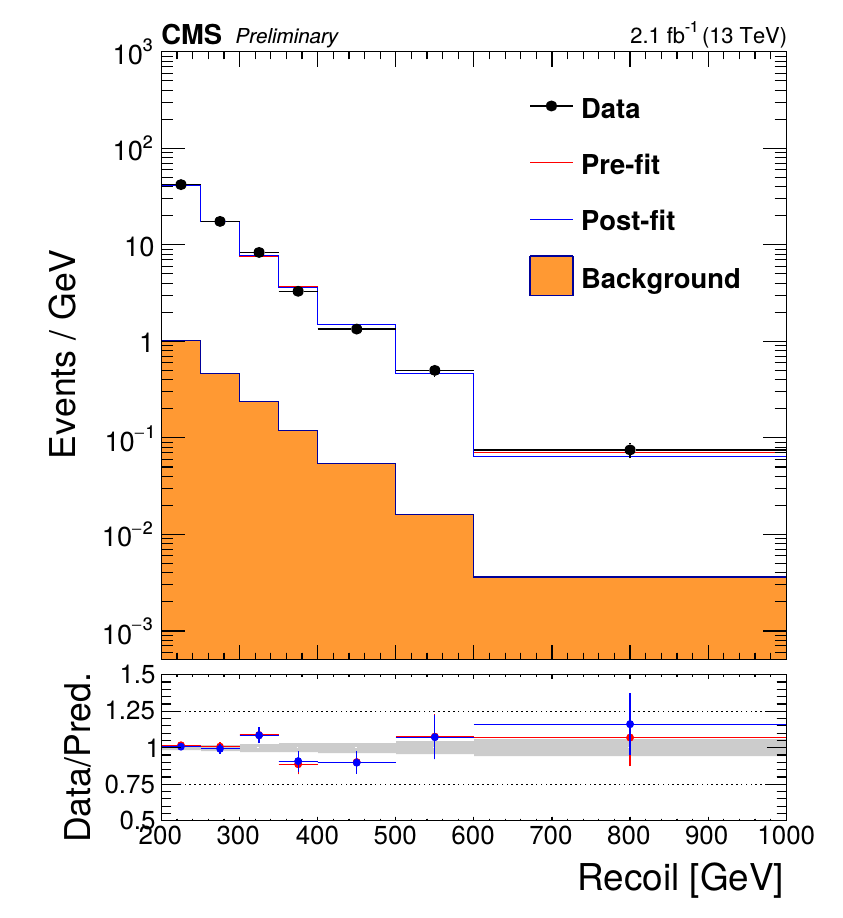
\includegraphics[width=.49\textwidth]{postfit_dimuon.png} 
%  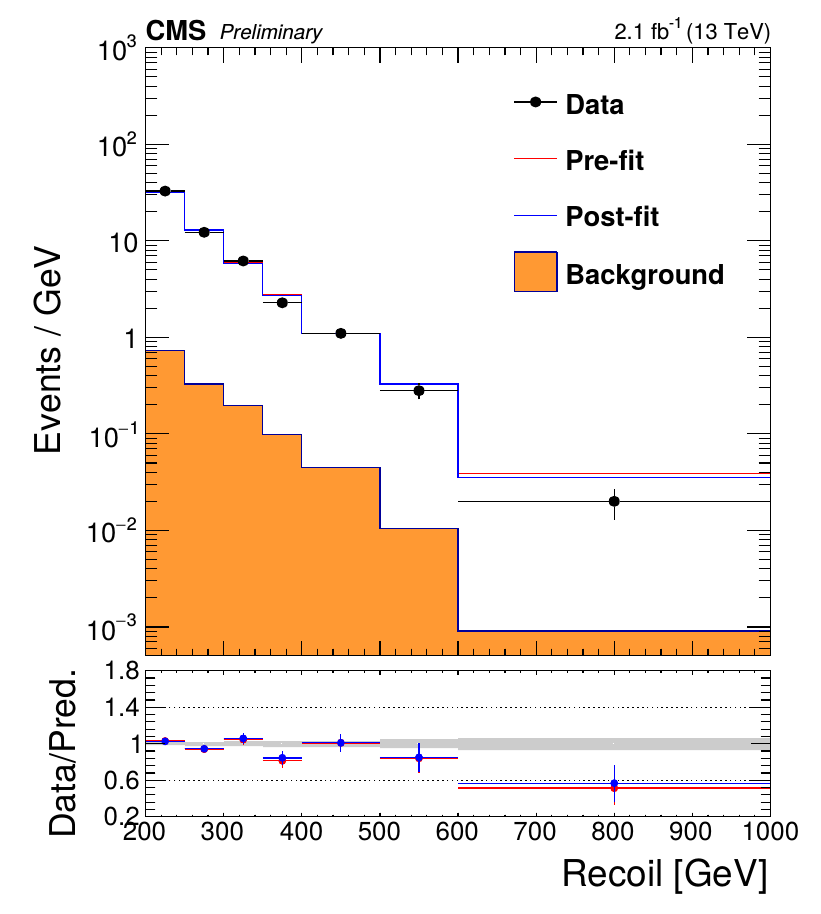
\includegraphics[width=.49\textwidth]{postfit_dielectron.png} \\
%  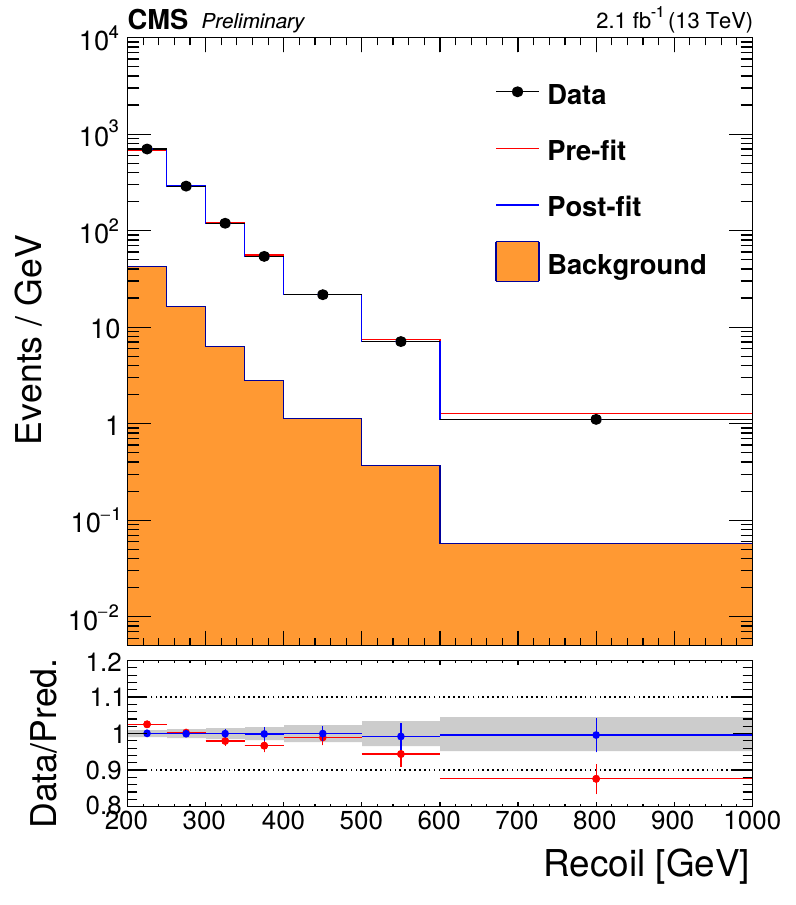
\includegraphics[width=.49\textwidth]{postfit_photon.png} 
%  \caption{Comparison between data and prediction before (pre-fit) and after (post-fit) the simultaneous fit to the different control regions, in the dimuon (left), dielectron (right) and photon + jets (bottom) control regions. The grey band shows the uncertainty per bin, including all relevant systematic uncertainties.}
%  \label{fig:postfit_1}
% \end{figure}
% 
% \begin{figure}[p]
%   \centering
%  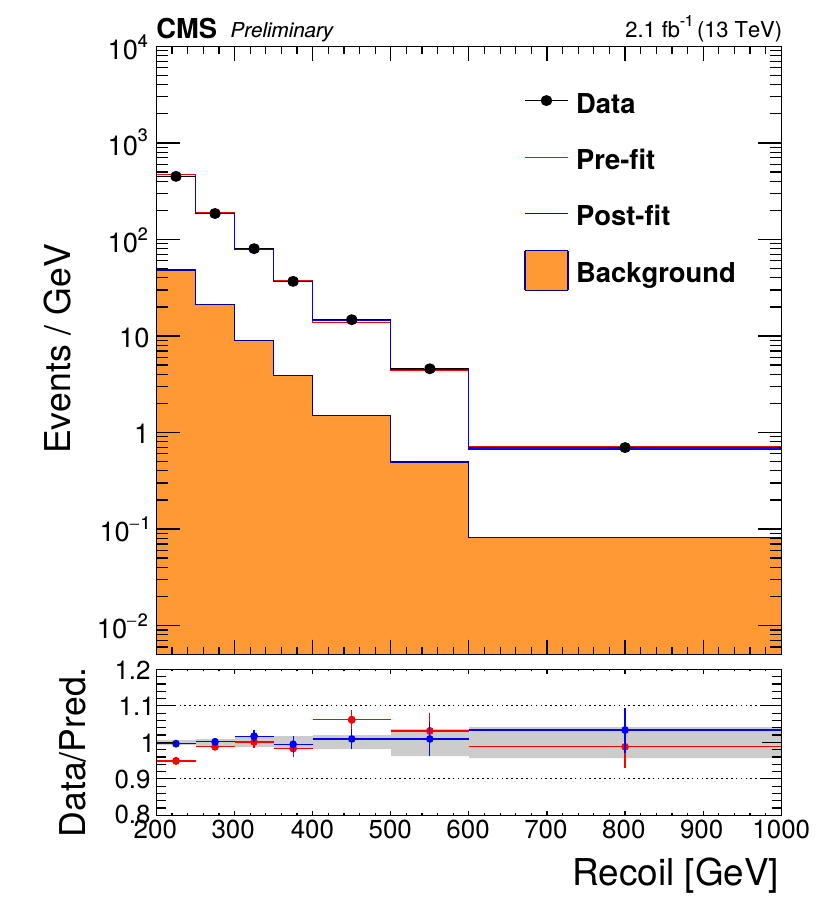
\includegraphics[width=.49\textwidth]{postfit_singlemuon.png} 
%  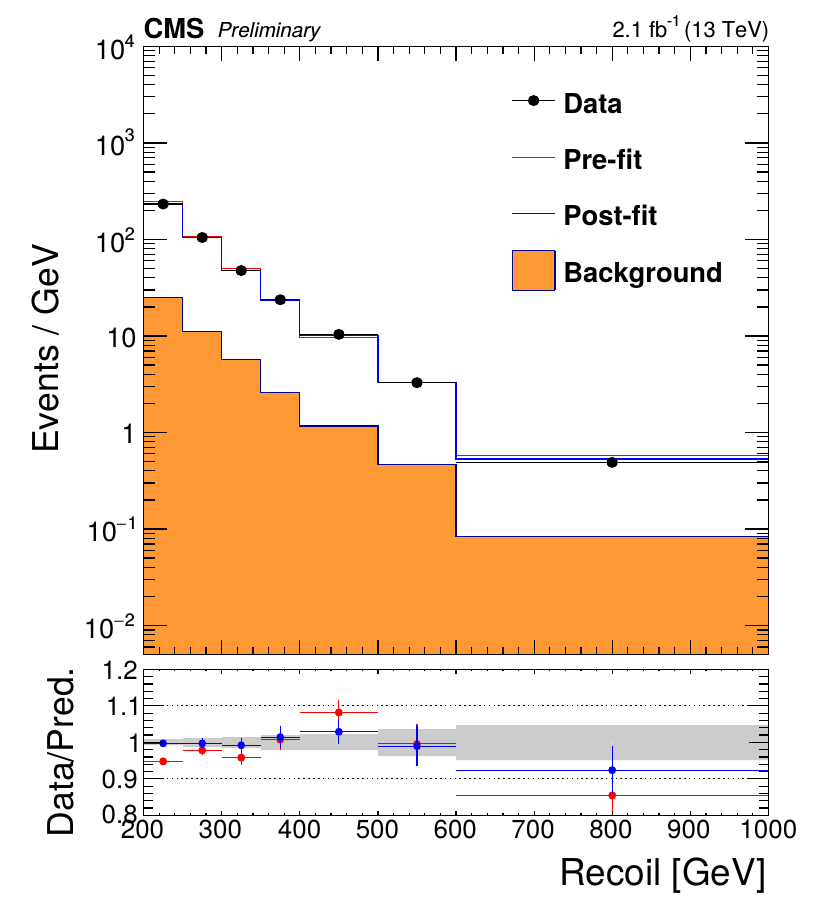
\includegraphics[width=.49\textwidth]{postfit_singleelectron.png}
%  \caption{Comparison between data and prediction before (pre-fit) and after (post-fit) the simultaneous fit to the single lepton control regions, in the single muon (left) and single electron (right) control regions. The grey band shows the uncertainty per bin, including all relevant systematic uncertainties.}
%  \label{fig:postfit_2}
% \end{figure}

Table~\ref{tab:monojet_yields_1} gives the background prediction for the various background processes in bins of hadronic recoil, using a background-only fit. Correspondingly, the fit under the background-only hypothesis is shown in Figure~\ref{fig:results} and a good agreement is observed between the data and the prediction. The uncertainty on the hadronic recoil is below 10\% for all bins.

% \begin{table}[ht]
%   \centering
%  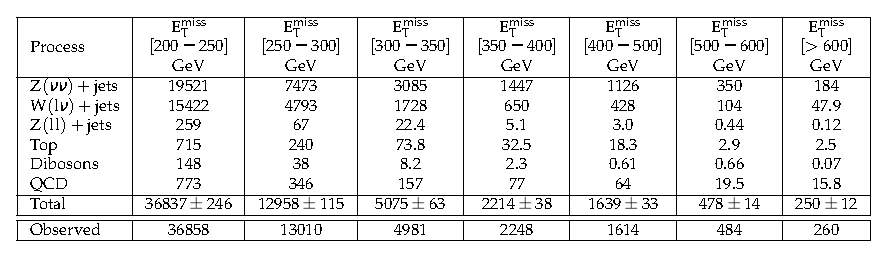
\includegraphics[width=\textwidth]{yields.pdf} 
%  \caption{Post-fit background predictions in the signal region and observed yield. The predictions and uncertainties are obtained from the background-only simultaneous fit in the signal and control regions.}
%  \label{tab:monojet_yields}
% \end{table}

\begin{landscape}

\begin{table}[ht]
  \centering
  \setlength{\tabcolsep}{3pt}
\caption{Pre-fit and post-fit background predictions in the signal region and observed yield given as number of events divided by the bin width, per $E_T^{miss}$ bin. The predictions and uncertainties are obtained from the background-only simultaneous fit in the signal and control regions.}
\label{tab:monojet_yields_1}
\scriptsize
\begin{subtable}{}
\renewcommand{\arraystretch}{1.2}
\begin{tabular}{| l | c | c | c | c | c | c | c | c | c | c | c | c |}
\hline
\multirow{3}{*}{process} &  $E_T^{miss}$ &  $E_T^{miss}$ &  $E_T^{miss}$ &  $E_T^{miss}$ &  $E_T^{miss}$ &  $E_T^{miss}$ &  $E_T^{miss}$ &  $E_T^{miss}$ &  $E_T^{miss}$ &  $E_T^{miss}$ &  $E_T^{miss}$ &  $E_T^{miss}$  \\
 & [200 - 230] & [230 - 260] & [260 - 290] & [290 - 320] & [320 - 350] & [350 - 390] & [390 - 430] & [430 - 470] & [470 - 510] & [510 - 550] & [550 - 590] & [590 - 640]  \\
 & GeV & GeV & GeV & GeV & GeV & GeV & GeV & GeV & GeV & GeV & GeV & GeV \\
\hline
  $Z(\nu\nu)$ + jets & 497 & 266 & 149 & 83.9 & 49.9 & 30.1 & 17.1 & 9.54 & 6.19 & 4.00 & 2.49 & 1.55\\
  $W(l\nu)$ + jets & 399 & 193 & 95.6 & 50.7 & 27.3 & 13.9 & 6.87 & 3.86 & 2.18 & 1.30 & 0.73 & 0.38\\
  $Z(ll)$ + jets & 6.88 & 3.10 & 1.26 & 0.61 & 0.33 & 0.10 & 0.05 & 0.02 & 0.01 & 0.01 & 0 & 0 \\
  top & 18.8 & 8.92 & 3.85 & 1.89 & 1.12 & 0.61 & 0.24 & 0.23 & 0.01 & 0.07 & 0.02 & 0\\
  QCD & 16.9 & 10.3 & 1.28 & 0.99 & 0.17 & 0.10 & 0.13 & 0.41 & 0.01 & 0 & 0.03 & 0\\
  dibosons & 8.36 & 5.23 & 2.58 & 1.43 & 0.85 & 0.55 & 0.35 & 0.17 & 0.13 & 0.05 & 0.05 & 0.03\\
  photon + jets & 7.67 & 3.36 & 2.12 & 0.99 & 0.66 & 0.32 & 0.21 & 0.12 & 0.09 & 0.05 & 0.05 & 0.01 \\
\hline
  total post-fit & 955 $\pm$ 6 & 489 $\pm$ 3 & 256 $\pm$ 2 & 141 $\pm$ 2 & 80.3 $\pm$ 1.2 & 45.7 $\pm$ 0.8 & 25.0 $\pm$ 0.6 & 14.4 $\pm$ 0.4 & 8.62 $\pm$ 0.32 & 5.49 $\pm$ 0.24 & 3.37 $\pm$ 0.17 & 1.97 $\pm$ 0.11 \\
\hline
  total pre-fit & 925 & 470 & 240 & 136 & 79.5 & 45.4 & 24.5 & 14.7 & 8.45 & 5.30 & 3.37 & 2.02\\
\hline
\hline
  observed & 953 & 492 & 259 & 140 & 78.8 & 46.9 & 25.2 & 13.6 & 8.73 & 5.40 & 3.55 & 2.22\\
\hline
\end{tabular}
\end{subtable}
\vspace*{.5cm}
% \caption{Pre-fit and post-fit background predictions in the signal region and observed yield. The predictions and uncertainties are obtained from the background-only simultaneous fit in the signal and control regions.}
% \label{tab:monojet_yields_2}
\begin{subtable}{}
\renewcommand{\arraystretch}{1.2}
\begin{tabular}{| l | c | c | c | c | c | c | c | c | c | c |}
\hline
\multirow{3}{*}{process} &  $E_T^{miss}$ &  $E_T^{miss}$ &  $E_T^{miss}$ &  $E_T^{miss}$ &  $E_T^{miss}$ &  $E_T^{miss}$ &  $E_T^{miss}$ &  $E_T^{miss}$ &  $E_T^{miss}$ &  $E_T^{miss}$  \\
 & [640 - 690] & [690 - 740] & [740 - 790] & [790 - 840] & [840 - 900] & [900 - 960] & [960 - 1020] & [1020 - 1090] & [1090 - 1160] & $> 1160$  \\
 & GeV & GeV & GeV & GeV & GeV & GeV & GeV & GeV & GeV & GeV \\
\hline
  $Z(\nu\nu)$ + jets & 0.90 & 0.56 & 0.44 & 0.27 & 0.16 & 0.09 & 0.06 & 0.04 & 0.02 & 0.02\\
  $W(l\nu)$ + jets & 0.22 & 0.12 & 0.11 & 0.06 & 0.03 & 0.02 & 0.01 & 0.01 & 0 & 0\\
  $Z(ll)$ + jets & 0 & 0 & 0 & 0 & 0 & 0 & 0 & 0 & 0 & 0\\
  top & 0 & 0 & 0 & 0.01 & 0 & 0 & 0 & 0 & 0 & 0\\
  QCD & 0.01 & 0 & 0 & 0 & 0 & 0 & 0 & 0 & 0 & 0\\
  dibosons & 0.03 & 0.01 & 0 & 0 & 0 & 0.01 & 0 & 0 & 0 & 0\\
  photon + jets  & 0 & 0.01 & 0.01 & 0 & 0 & 0 & 0 & 0 & 0 & 0\\
\hline
  total post-fit & 1.16 $\pm$ 0.08 & 0.70 $\pm$ 0.05 & 0.55 $\pm$ 0.05 & 0.34 $\pm$ 0.04 & 0.20 $\pm$ 0.02 & 0.11 $\pm$ 0.02 & 0.07 $\pm$ 0.02 & 0.05 $\pm$ 0.01 & 0.03 $\pm$ 0.01 & 0.02 $\pm$ 0.01\\
\hline
  total pre-fit  & 1.19 & 0.73 & 0.48 & 0.31 & 0.20 & 0.13 & 0.09 & 0.05 & 0.03 & 0.02\\
\hline
\hline
  observed & 1.22 & 0.64 & 0.56 & 0.28 & 0.22 & 0.12 & 0.05 & 0.01 & 0.03 & 0.03 \\
\hline
\end{tabular}
\end{subtable}
\end{table}

\end{landscape}

\begin{figure}[ht]
  \centering
 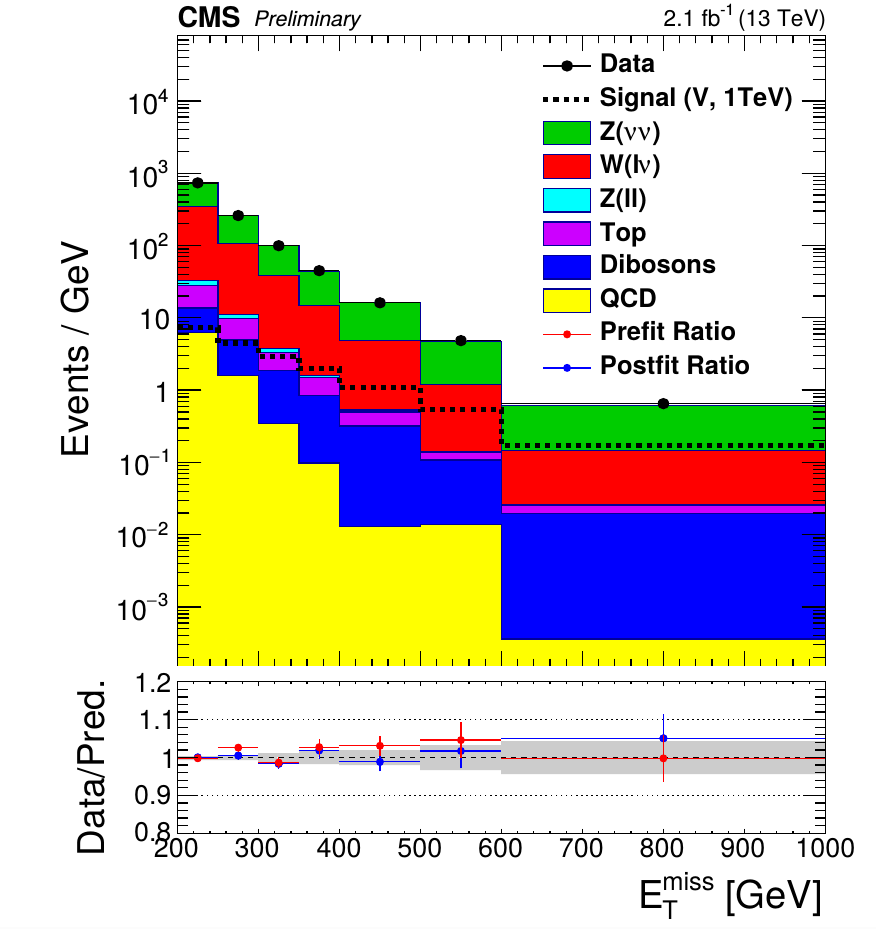
\includegraphics[width=.7\textwidth]{results.png} 
 \caption{Post-fit missing transverse momentum distribution for the expected backgrounds and the observed data in the signal region. The grey band indicates the post-fit uncertainty obtained from the background-only simultaneous fit in the signal and control regions.}
 \label{fig:results}
\end{figure}

\section{Improvements going from the 2015 to the 2016 analysis}
\label{sec:improvement}

Several iterations of the monojet analysis were performed during Run 2 in 2015 and 2016, improving the achieved sensitivity with the increase in available data and additional developments to the analysis strategy, and adding new interpretations. In 2015, a first analysis with data at a centre-of-mass energy of \SI{13}{TeV} was carried out~\cite{CMS:2015jdt}, using data corresponding to an integrated luminosity of $2.1\ \mathrm{fb}^{-1}$. In this first iteration of the search, the NLO k-factors applied to correct the \ac{LO} samples used for the estimation of the background from $Z$ and $W$ bosons are derived from inclusive \ac{NLO} samples, which are not binned in boson $p_T$. These k-factors are shown in Figure~\ref{fig:kfactors_15}, and can be compared to the k-factors obtained from $p_T$-binned samples used in the following iterations of the analysis and shown in Figure~\ref{fig:kfactors}.

\begin{figure}[ht]
  \centering
 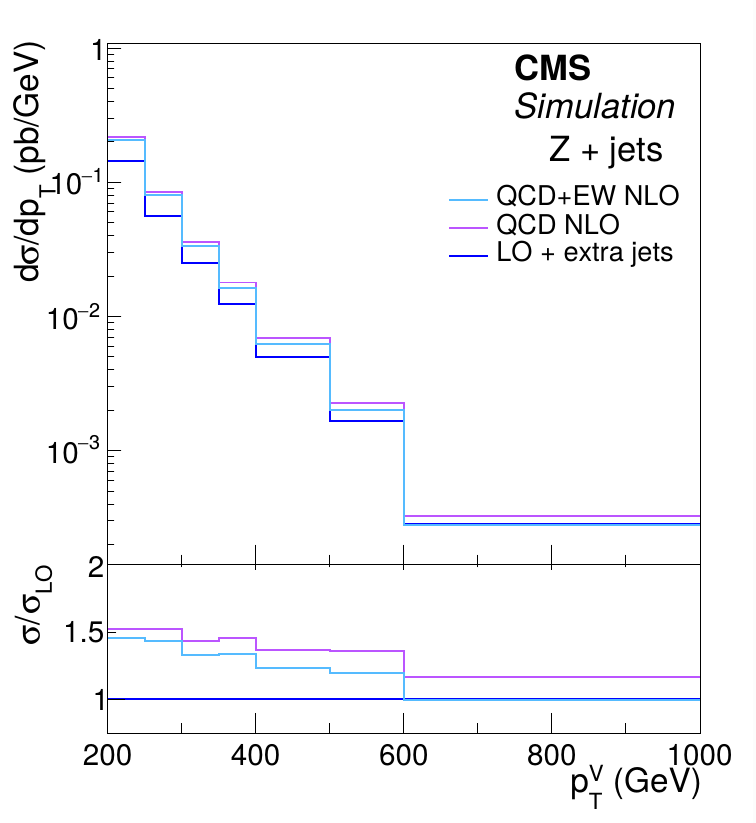
\includegraphics[width=.49\textwidth]{Z_kfactor.png} 
 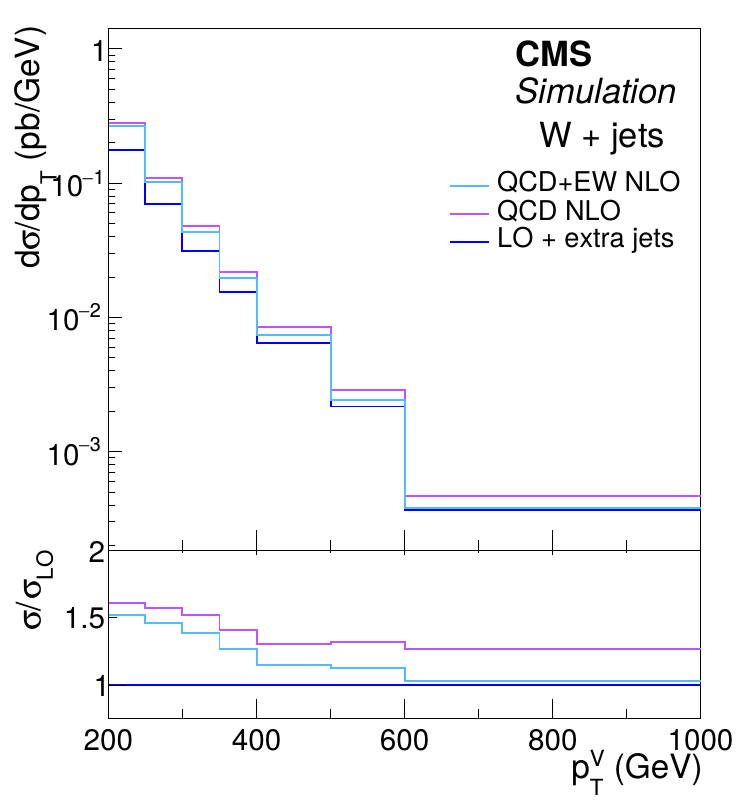
\includegraphics[width=.49\textwidth]{W_kfactor.png} \\
 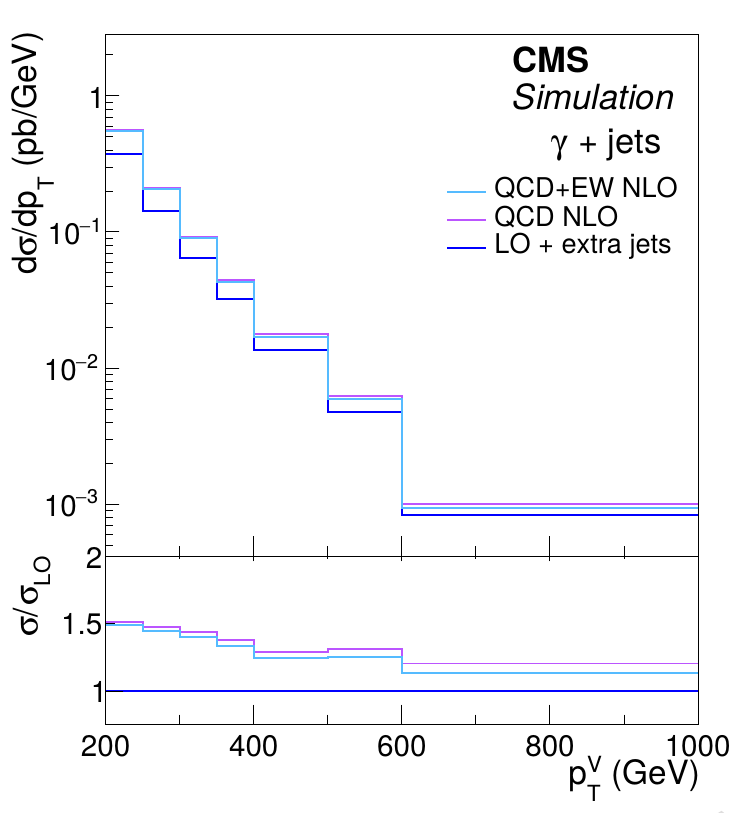
\includegraphics[width=.49\textwidth]{gamma_kfactor.png} 
 \caption{The differential cross section as a function of the boson $p_T$ for photon, $W$, and $Z$ production, using inclusive \ac{NLO} samples. The resulting k-factors are shown in the ratio plots.}
 \label{fig:kfactors_15}
\end{figure}

In 2016, the analysis was extended to the mono-V channel~\cite{CMS:2016tns}, which can give rise to a monojet-like signature. At high $p_T$, the production of a $W$ or $Z$ boson which decays hadronically, can be effectively reconstructed as a single jet of large cone radius. However, in this chapter the focus is on the monojet channel and the added improvements during 2016. For this analysis, data collected in 2015 was used, corresponding to $2.3\ \mathrm{fb}^{-1}$. This is the analysis reported in this chapter.  The used \ac{NLO} k-factors were derived using the $p_T$-binned samples, as described in Section~\ref{sec:main_bkgd}. This contribution was a first step in the improvements I added to the analysis. I performed extensive validations, comparing the obtained k-factors to the previous results. 

A substantial difference in the next iteration of the 2016 analysis~\cite{Sirunyan:2017hci} is the increase in collected data, which allowed to reduce the statistical uncertainties and set stronger limits on the considered models. For these results, data collected in the first half of 2016 and corresponding to an integrated luminosity of $12.9\ \mathrm{fb}^{-1}$ were available. One of the improvements that were added is the direct use of MC samples generated at next-to-leading order for the estimation of the main backgrounds. This was possible by generating larger samples that are binned in $W$ boson $p_T$, and are now used more widely in other analyses. As a result of my second contribution to the improvement of the background prediction, no k-factors need to be applied to the $W$ + jets sample and no additional systematic uncertainties are to be introduced for this. Figures~\ref{fig:comparison} and~\ref{fig:comparison2} show the obtained reduction in the overall post-fit uncertainty on the predictions in the 5 control regions, which is clearly visible at high missing transverse momentum. The largest uncertainties of about 50\% in the high $E_T^{miss}$ region are reduced to 20\% or less, which is driving the analysis sensitivity at the highest mediator masses.

\begin{figure}[p]
  \centering
 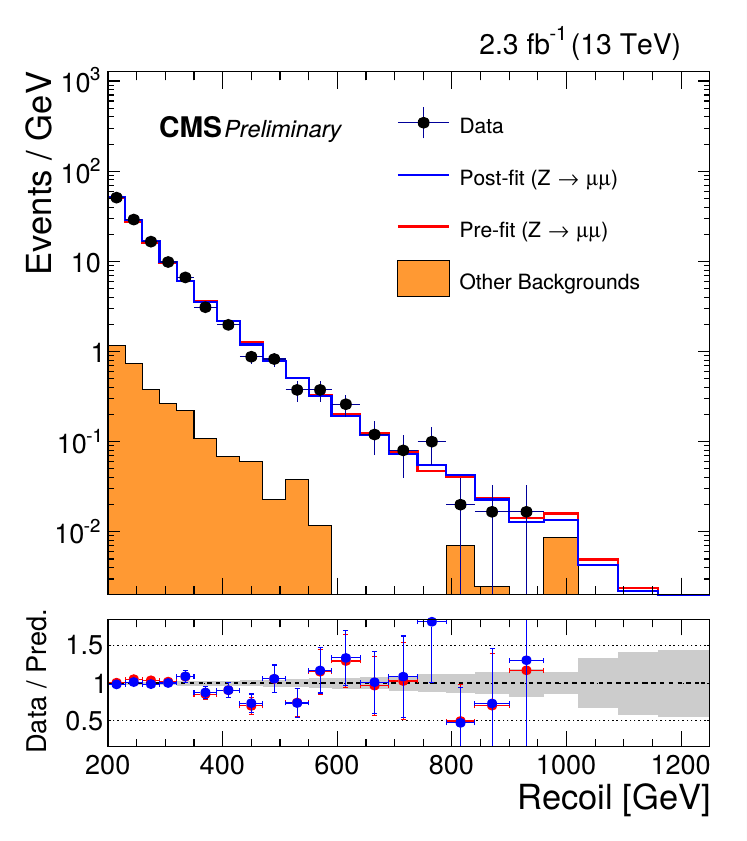
\includegraphics[width=.38\textwidth]{EXO-16-013_dimuon.png} \hspace{.35cm}
 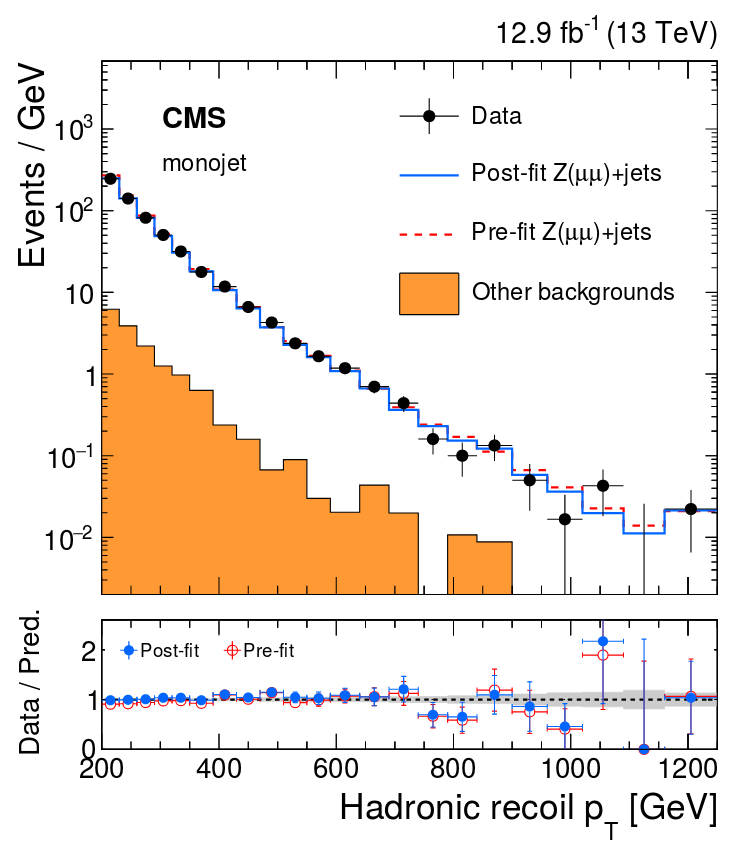
\includegraphics[width=.38\textwidth]{EXO-16-037_dimuon.png} \\
 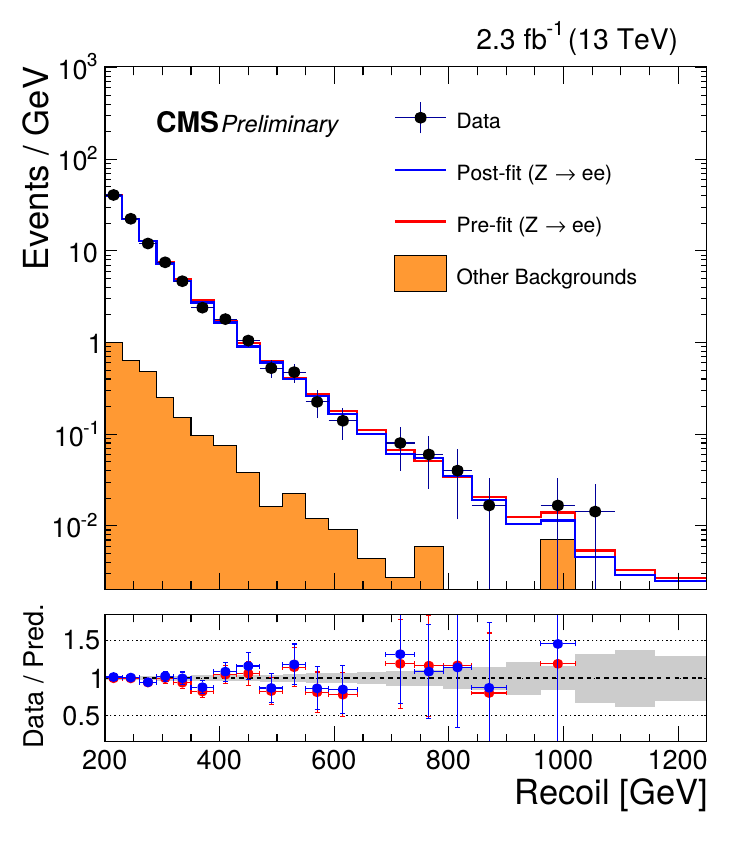
\includegraphics[width=.38\textwidth]{EXO-16-013_dielectron.png} \hspace{.35cm}
 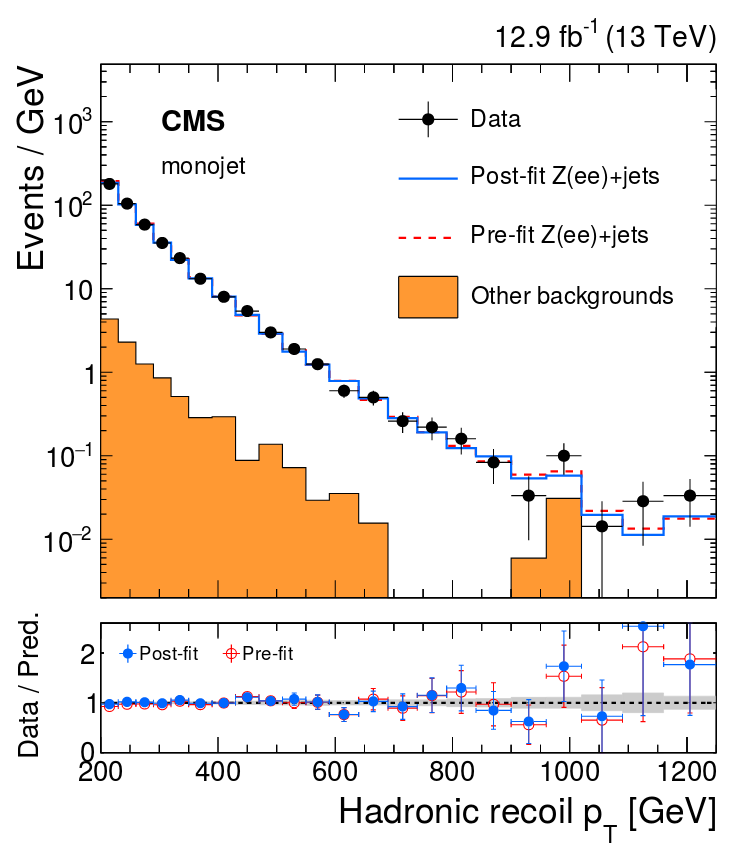
\includegraphics[width=.38\textwidth]{EXO-16-037_dielectron.png} \\
 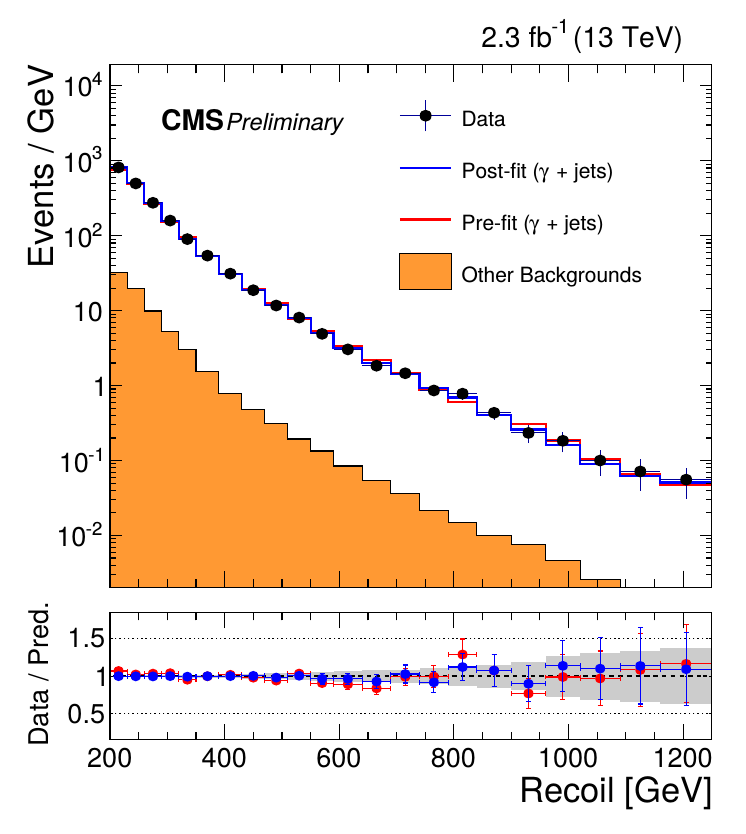
\includegraphics[width=.38\textwidth]{EXO-16-013_gamma.png}  \hspace{.35cm}
 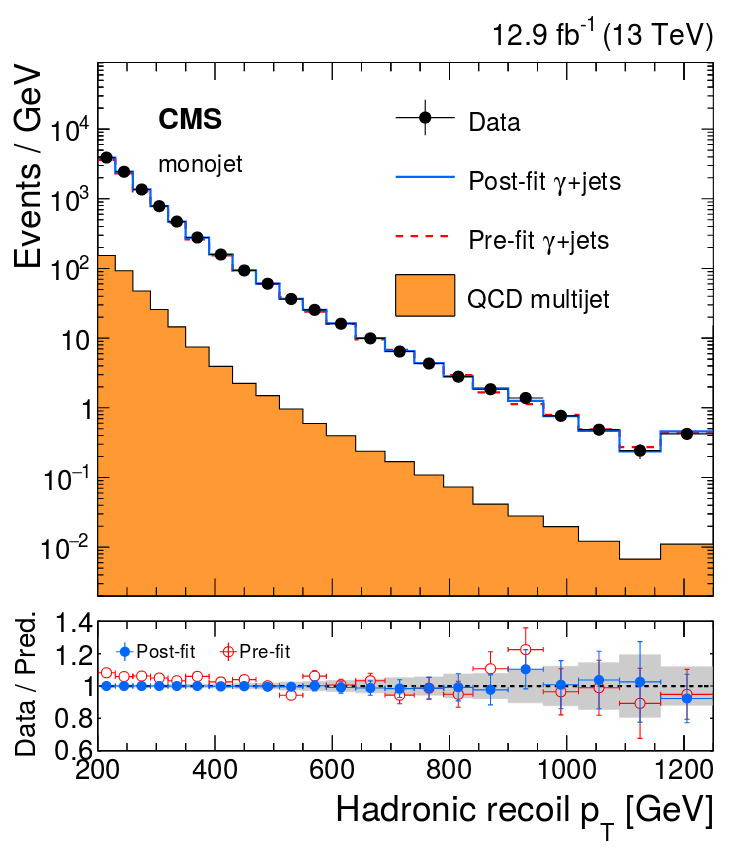
\includegraphics[width=.38\textwidth]{EXO-16-037_gamma.png} 
 \caption{Comparison of the hadronic recoil $p_T$ distribution between the data and MC simulation in the dimuon (top), dielectron (middle), and photon + jets (bottom) control regions, showing the reduction in overall post-fit uncertainty (grey band) going from the early 2016 analysis (left) to the analysis using data from the first half of 2016 (right). The fit was performed simultaneously over all the control and signal regions, assuming the absence of any signal. The last bin includes all events with hadronic recoil $p_T > \SI{1160}{GeV}$. Figures taken from~\cite{CMS:2016tns} and~\cite{Sirunyan:2017hci}.}
 \label{fig:comparison}
\end{figure}

\begin{figure}[p]
  \centering
 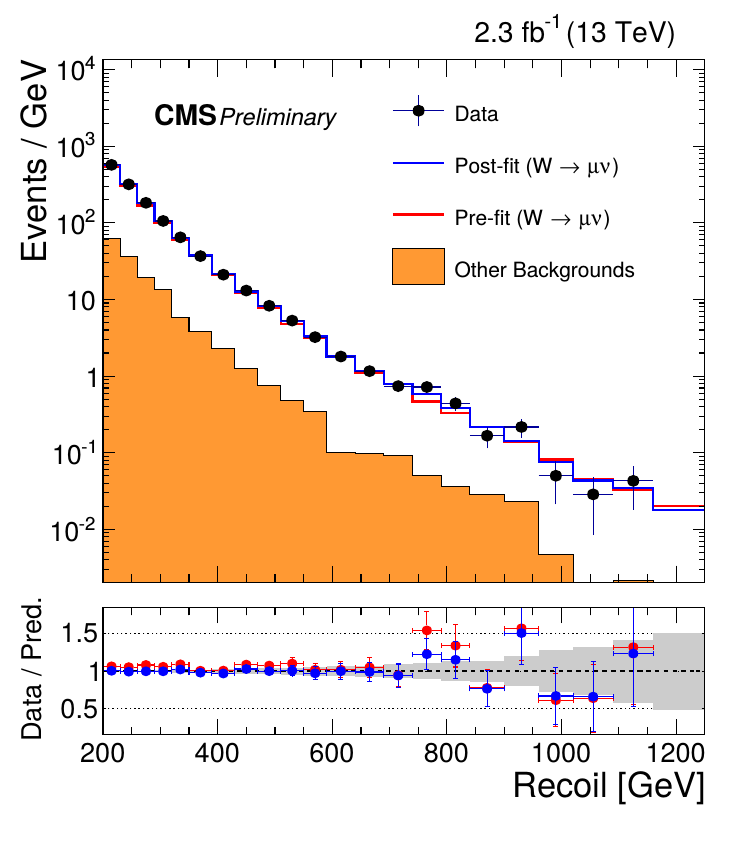
\includegraphics[width=.4\textwidth]{EXO-16-013_singlemuon.png}  \hspace{.35cm}
 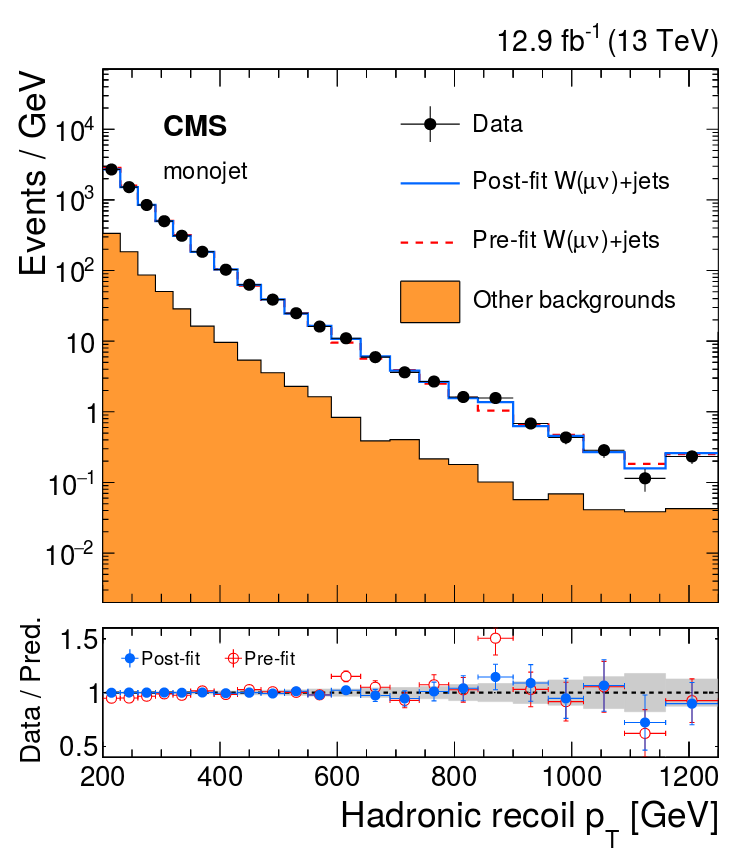
\includegraphics[width=.4\textwidth]{EXO-16-037_singlemuon.png} \\
 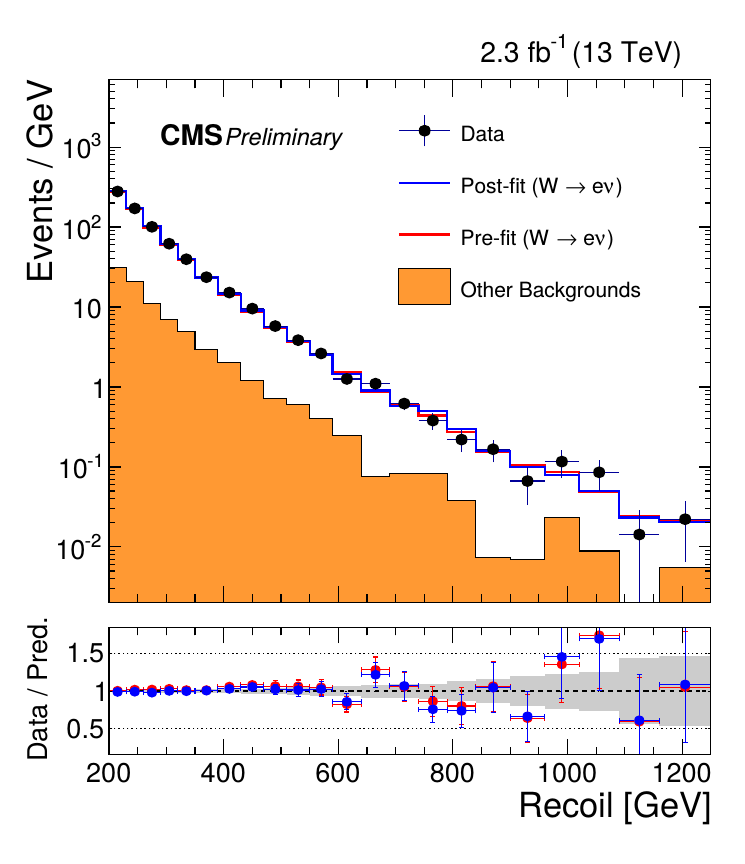
\includegraphics[width=.4\textwidth]{EXO-16-013_singleelectron.png}  \hspace{.35cm}
 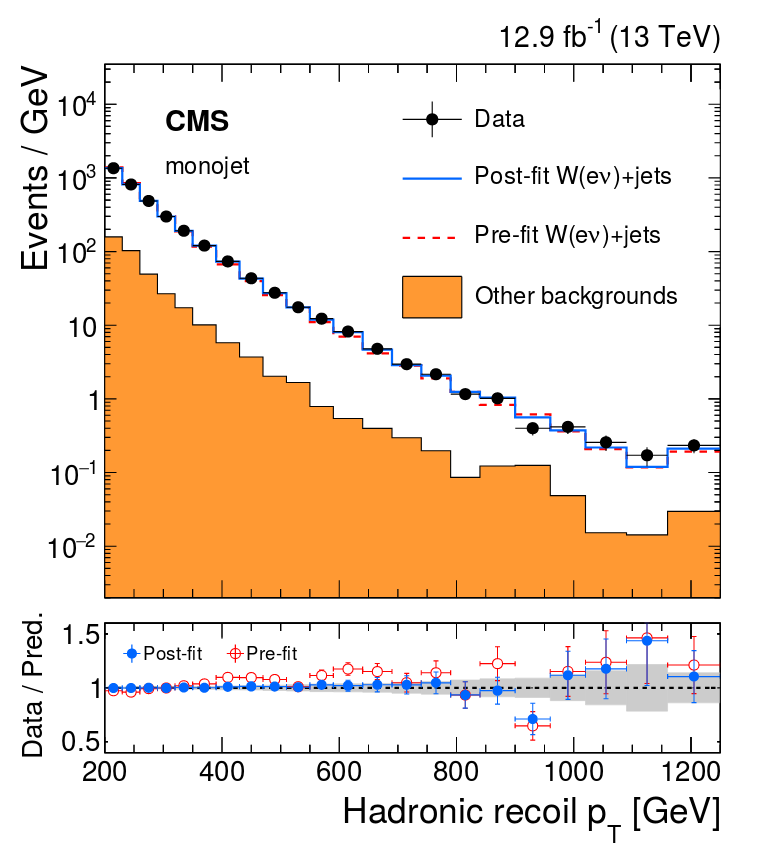
\includegraphics[width=.4\textwidth]{EXO-16-037_singleelectron.png} \\
 \caption{Comparison of the hadronic recoil $p_T$ distribution between the data and MC simulation in the single muon (top) and single electron (bottom) control regions, showing the reduction in overall post-fit uncertainty (grey band) going from the early 2016 analysis (left) to the analysis using data from the first half of 2016 (right). The fit was performed simultaneously over all the control and signal regions, assuming the absence of any signal. The last bin includes all events with hadronic recoil $pT > \SI{1160}{GeV}$. Figures taken from~\cite{CMS:2016tns} and~\cite{Sirunyan:2017hci}.}
 \label{fig:comparison2}
\end{figure}

\section{Limit setting}
\label{sec:limits}

As no significant excess was observed, upper limits are placed on the ratio of the signal cross section to the predicted cross section. This limit setting on new physics models is done with respect to the signal plus background hypothesis, comparing it to the background only hypothesis in which no new physics is present. Typically, a specific variable, for which different outcomes are predicted in the different hypotheses, is used to build a test statistic. The distribution of the test statistic is constructed by generating pseudo-experiments for each hypothesis. In case the expected number of events is large, the asymptotic approximation~\cite{Cowan:2010js} is used to reduce the large computing time, replacing the pseudo-experiments by a single so-called Asimov data set.

The $CL_S$ method~\cite{CLS1,CLS2} is then used to determine the compatibility of the signal hypothesis with the observed data and to derive the upper limits at a certain confidence level (CL). In this thesis, the \ac{LHC} style test statistic~\cite{ATLAS:2011tau} is used, given by
\begin{equation}
 q_{\mu} = -2 \ln \frac{\mathcal{L}\left(data|\mu, \hat{\theta}_{\mu} \right)}{\mathcal{L}\left( data|\hat{\mu}, \hat{\theta} \right)} \quad \left(0 \leq \hat{\mu} \leq \mu\right),
\end{equation}
where $\mu$ is the signal strength, $\theta_{\mu}$ are the nuisance parameters for a given $\mu$, $\hat{\mu}$ is the maximum likelihood value of $\mu$, and $\hat{\theta}_{\mu}$ are the corresponding nuisance parameters. The signal strength represents the fraction of the theoretical cross section corresponding to the considered hypothesis. When constructing the distribution of the used variable, the expected number of events in the $i$-th bin is then $\mu s_i + b_i$, with $s_i$ and $b_i$ the number of predicted signal and background events in that bin. $\mu = 0$ thus corresponds to the background only hypothesis, and $\mu = 1$ corresponds to the signal plus background hypothesis using the nominal theoretical cross section.

Adding a given observation of the test statistic, $q_{\mu, obs}$, from a measurement in data, the probability to find a data set with value of the test statistic equal or larger under the signal plus background hypothesis can be written as
\begin{equation}
 p_{s+b} = \int_{q_{\mu, obs}}^{\infty} f_{s+b}\left( q_{\mu}|\mu \right)dq_{\mu},
\end{equation}
where $ f_{s+b}\left( q_{\mu}|\mu \right)$ is the probability density function of the signal plus background hypothesis constructed from the pseudo-experiments. Similarly, the probability to find a data set equally or more incompatible with the background only hypothesis is given by
\begin{equation}
 1 - p_b = \int^{q_{\mu, obs}}_{-\infty} f_b\left( q_{\mu}|0 \right)dq_{\mu}.
\end{equation}
In these equations, $p_{s+b}$ and $p_b$ are the p-values associated to the two hypotheses. The $CL_S$ value, which represents the compatibility of the signal hypothesis with the observed data, is defined as the ratio of these two probabilities:
\begin{equation}
 CL_S = \frac{p_{s+b}}{1 - p_b}
\end{equation}
Models can then be considered to be excluded at 95\% CL when $CL_S \leq 0.05$.

\section{Interpretation}
\label{sec:interpretation}

The results of the second iteration of this search, using the mono-V final state as well, are interpreted in terms of simplified dark matter models assuming a vector, axial-vector, scalar, or pseudoscalar mediator decaying to a pair of fermionic dark matter particles, as described in Section~\ref{sec:monojet_models}. As no significant excess was observed, upper limits are placed at 95\% confidence level (CL) on the ratio of the signal cross section to the predicted cross section, $\mu = \sigma/\sigma_{th}$, following the method described in Section~\ref{sec:limits}. These limits are shown as a function of the mediator mass ($m_{\mathrm{med}}$) and the dark matter mass ($m_{\mathrm{DM}}$) in Figures~\ref{fig:limits_1} and \ref{fig:limits_2}, for the four types of mediators. The regions where the 95\% CL upper limits on $\mu$ are less than one are considered to be excluded.


\begin{figure}[ht]
  \centering
 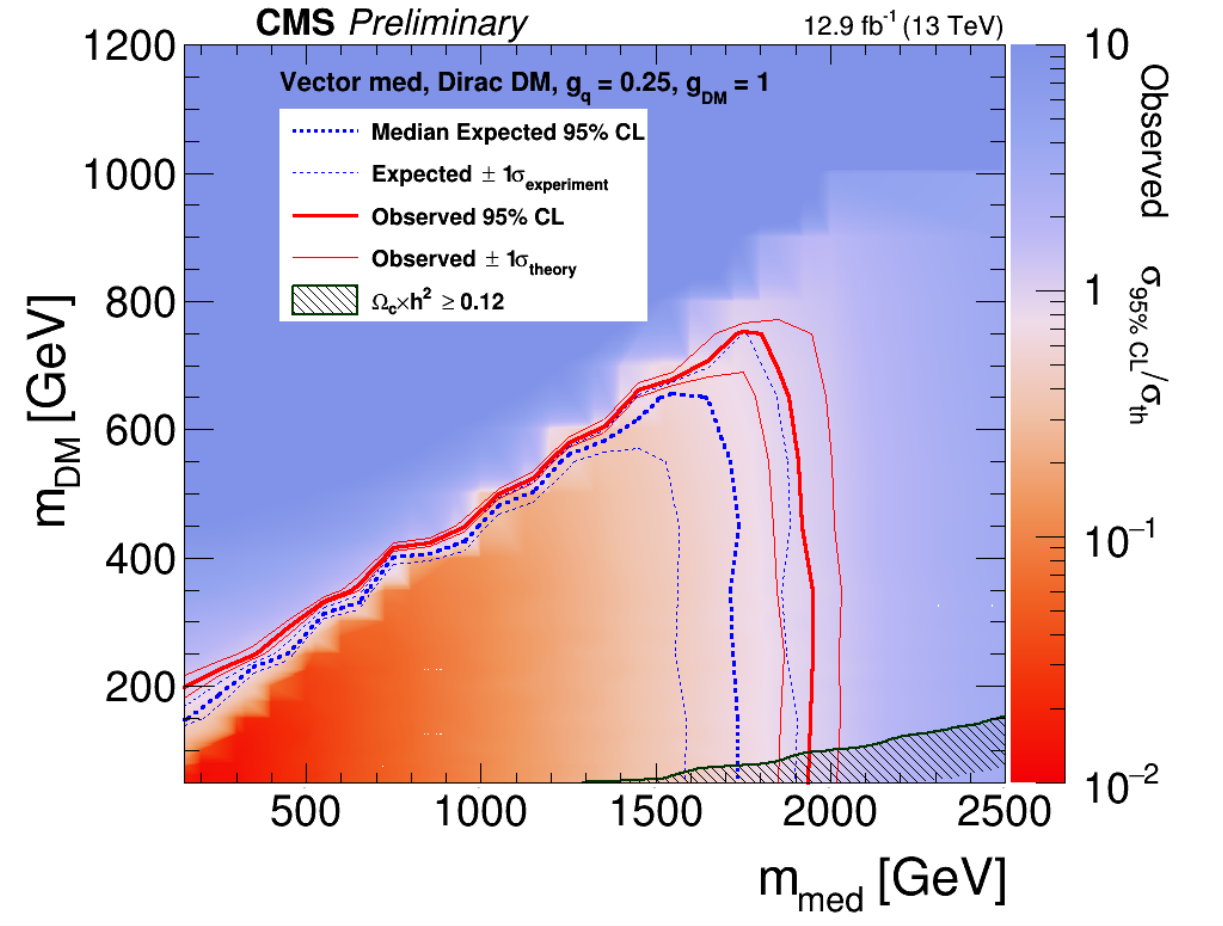
\includegraphics[width=.49\textwidth]{vectormed.png} 
 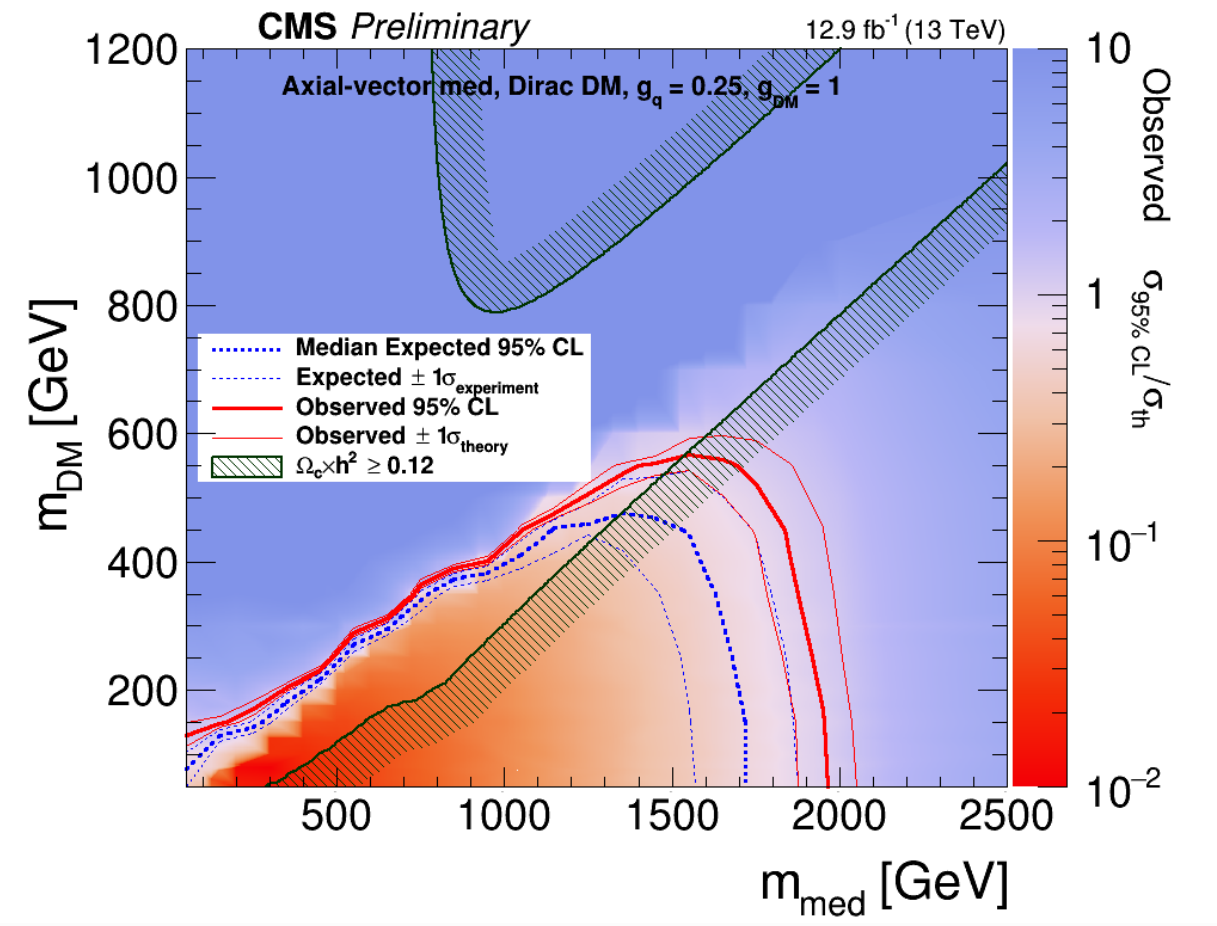
\includegraphics[width=.49\textwidth]{axialmed.png} 
 \caption{The 95\% CL upper limits on the $\mu =  \sigma/\sigma_{th}$ in the  $m_{\mathrm{med}}-m_{\mathrm{DM}}$ plane, for a vector (left) or axial-vector (right) mediator. The cosmological constraints from the WMAP and Planck measurements of the \ac{CMB} are shown as well. Figures taken from~\cite{Sirunyan:2017hci}.}
 \label{fig:limits_1}
\end{figure}

\begin{figure}[ht]
  \centering
 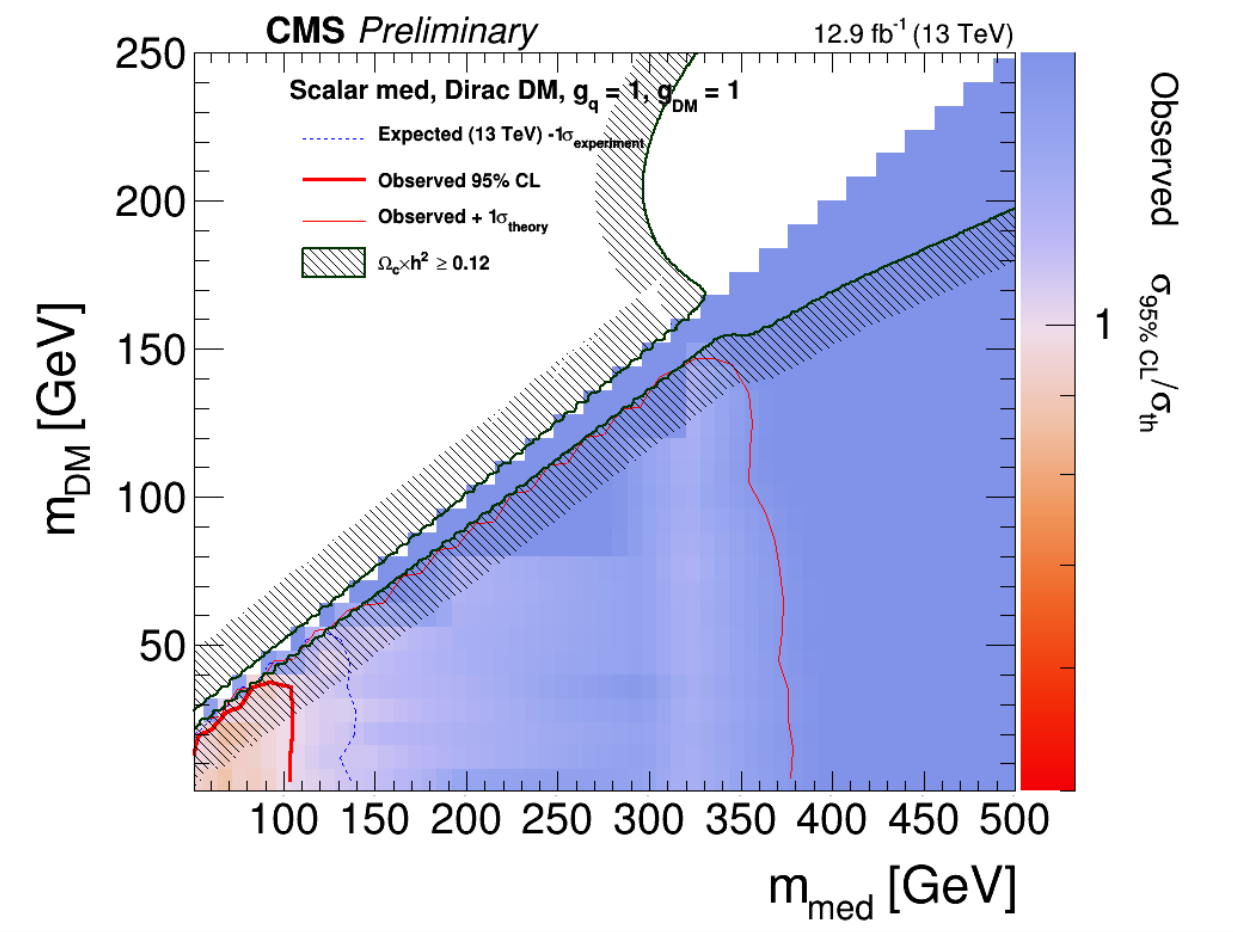
\includegraphics[width=.49\textwidth]{scalarmed.png} 
 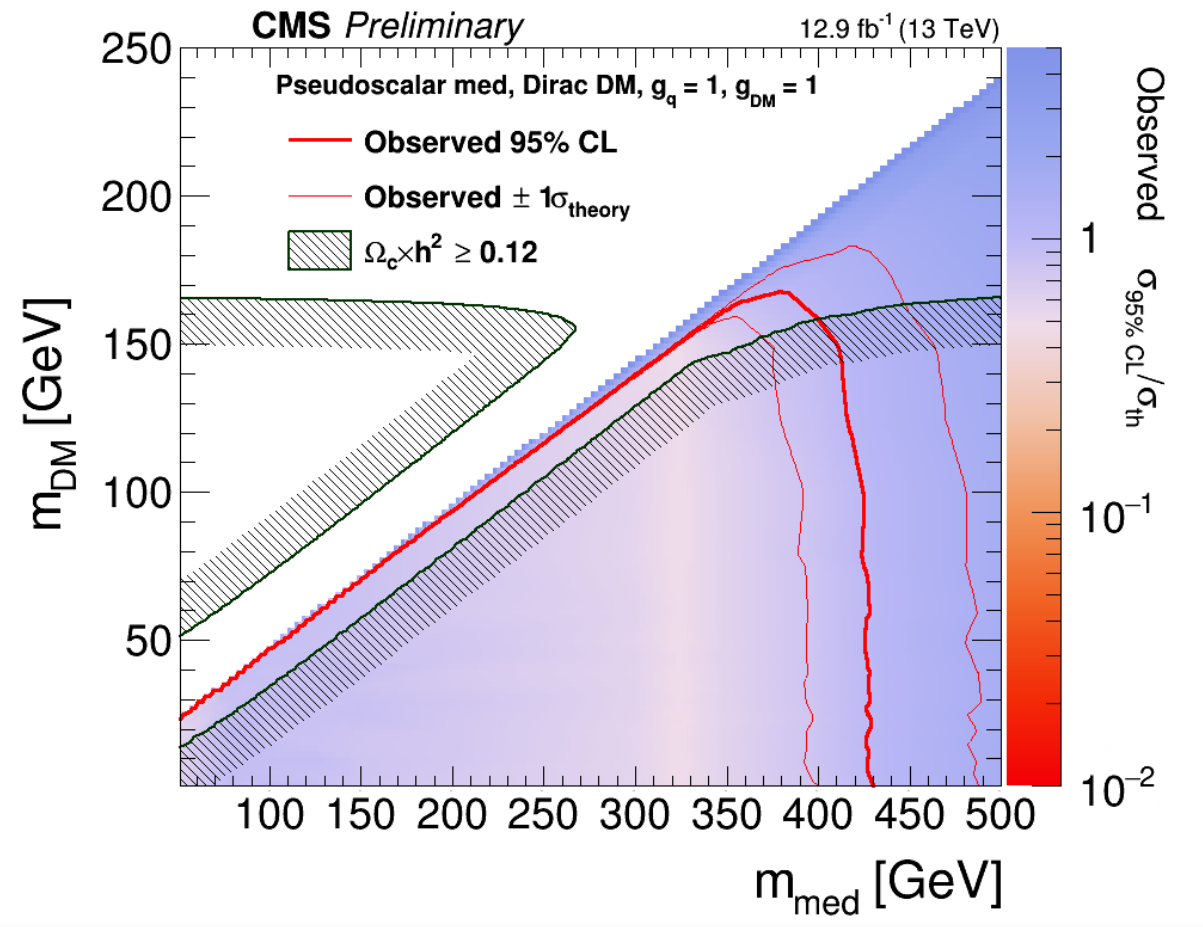
\includegraphics[width=.49\textwidth]{pseudoscalarmed.png} 
 \caption{The 95\% CL upper limits on the $\mu =  \sigma/\sigma_{th}$ in the  $m_{\mathrm{med}}-m_{\mathrm{DM}}$ plane, for a scalar (left) or pseudoscalar (right) mediator. The cosmological constraints from the WMAP and Planck measurements of the \ac{CMB} are shown as well. Figures taken from~\cite{Sirunyan:2017hci}.}
 \label{fig:limits_2}
\end{figure}

For the vector and axial-vector models, mediator masses up to \SI{1.95}{TeV} are excluded, while mediator masses up to \SI{100}{GeV} and \SI{430}{GeV} can be excluded for the scalar and pseudoscalar models, respectively. Figures~\ref{fig:limits_1} and \ref{fig:limits_2} also show the constraint from the observed cosmological relic density of dark matter, which was determined from the WMAP and Planck \ac{CMB} measurements. The expected dark matter abundance is estimated using a thermal freeze-out mechanism and compared to the observed cold dark matter density, assuming that the considered dark matter candidate is the dominant component of the observed dark matter.

The obtained limits can also be translated into 90\% CL upper limits on the dark matter-nucleon scattering cross section $\sigma_{\mathrm{SI/SD}}$, in order to compare them to results from direct detection experiments. The exclusion contours in the $m_{\mathrm{DM}}-\sigma_{\mathrm{SI/SD}}$ plane are obtained following the approaches outlined in \cite{Buchmueller:2014yoa, Kurylov:2003ra, Hisano:2010ct}, where $\sigma_{\mathrm{SI}}$ stands for spin-independent and $\sigma_{\mathrm{SD}}$ for spin-dependent dark matter-nucleon cross section. The resulting limits are shown in Figures~\ref{fig:DDlimits_1} and \ref{fig:DDlimits_2}.

\begin{figure}[ht]
  \centering
 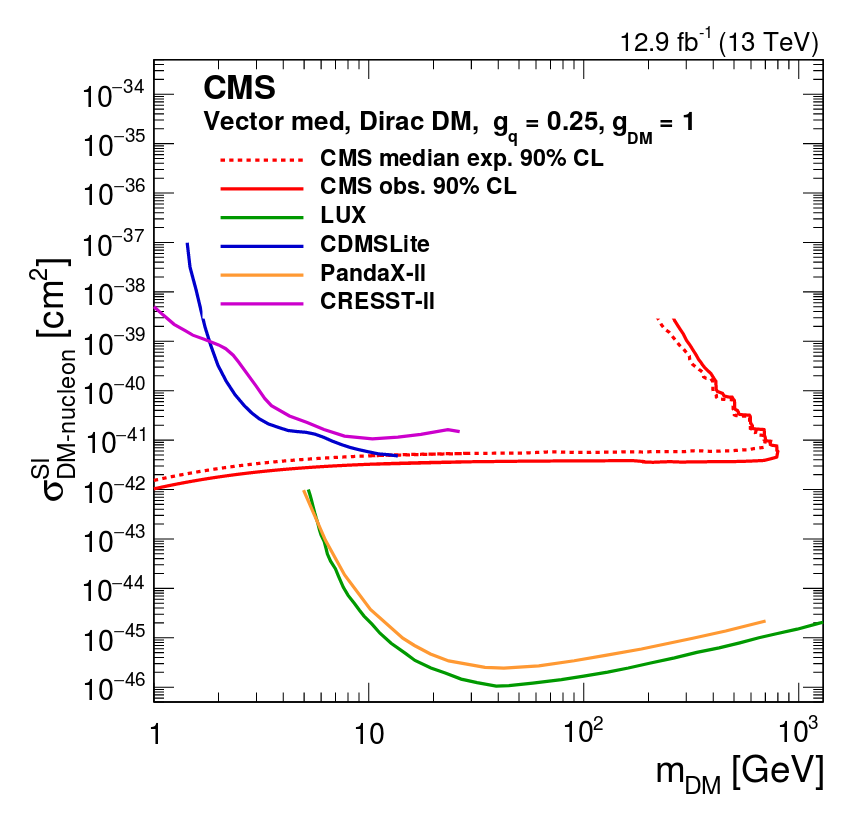
\includegraphics[width=.49\textwidth]{vector_DD.png} 
 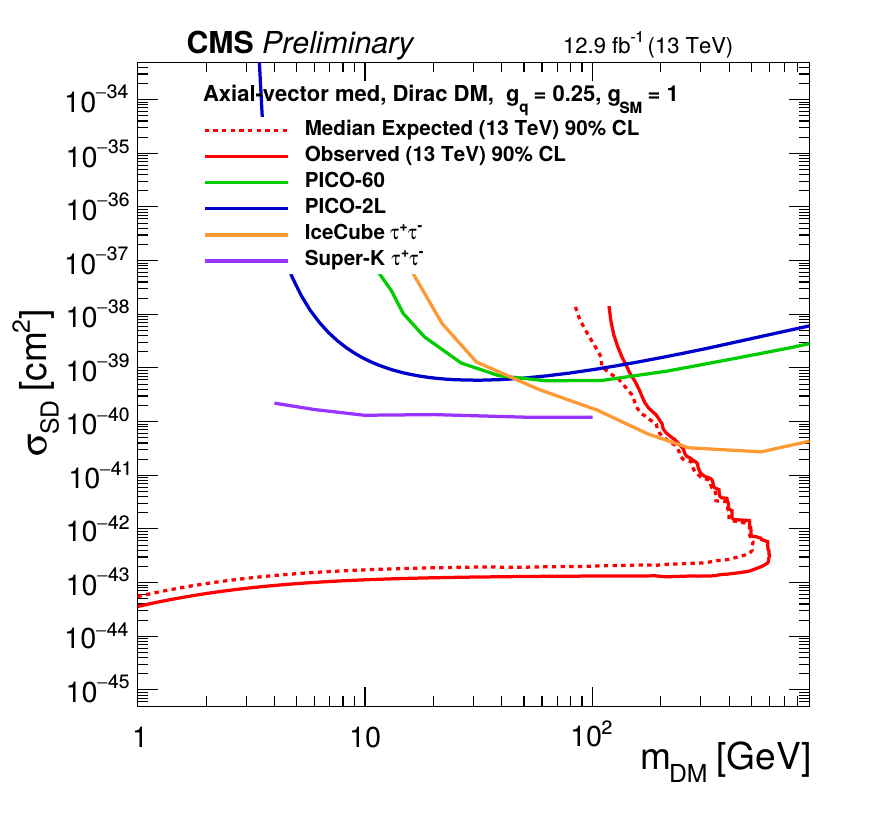
\includegraphics[width=.49\textwidth]{axial_DD.png} 
 \caption{The 90\% CL upper limits in the  $m_{\mathrm{DM}}-\sigma_{\mathrm{SI/SD}}$ plane, for a vector (left) or axial-vector (right) mediator. Figures taken from~\cite{Sirunyan:2017hci}.}
 \label{fig:DDlimits_1}
\end{figure}

\begin{figure}[ht]
  \centering
 \includegraphics[width=.49\textwidth]{scalar_DD.png} 
 \includegraphics[width=.49\textwidth]{pseudoscalar_DD.png} 
 \caption{The 90\% CL upper limits in the  $m_{\mathrm{DM}}-\sigma_{\mathrm{SI/SD}}$ plane, for a scalar (left) or pseudoscalar (right) mediator. Figures taken from~\cite{Sirunyan:2017hci}.}
 \label{fig:DDlimits_2}
\end{figure}

For the vector and scalar mediator cases, the derived 90\% CL upper limits on the spin-independent cross section are compared to the results from the CDMSLite~\cite{Agnese:2015nto}, LUX~\cite{Akerib:2015rjg}, CRESST-II~\cite{Angloher:2015ewa}, and PandaX-II~\cite{Tan:2016zwf} experiments. This shows that the monojet limits are complementary to the results from the direct detection experiments at low dark matter masses. The 90\% CL upper limits on the spin-dependent cross section for the axial-vector mediator are compared to the PICO-2L~\cite{Amole:2016pye}, PICO-60~\cite{Amole:2015pla}, Super Kamiokande~\cite{Choi:2015ara}, and IceCube~\cite{Aartsen:2016exj} experiments. In the case of the pseudoscalar mediator, the obtained limits are compared to the indirect detection results from the Fermi-LAT experiment~\cite{Ackermann:2011wa,Abdo:2010ex}. In the considered scenario the dark matter annihilates into $b$ quark pairs in the centre of the galaxy, producing gamma rays.

\section{Summary}

The monojet analysis has been detailed in this chapter, focusing on the monojet channel and omitting the mono-V channel. The background estimation is emphasised, as this is the aspect the author contributed to. The theoretical and statistical uncertainties were significantly reduced in the subsequent iterations by adding the discussed improvements, enhancing the sensitivity of the analysis. No excess was observed above the expected background, and the obtained results allow the exclusion of a larger phase space for the considered models.

\clearpage{\pagestyle{empty}\cleardoublepage}
